%!TEX root = ../Thesis.tex

\chapter{Prototype}
The ground control platform must have some physical dimension due to the size of the UAV used in this project. The dimension of the UAV used will effect the dimension and choice of construction of the ground station. In dimensioning and designing the ground station the primary focus is on making an industrial and robust prototype. 


\section{Landing platform / Helipad}
The landing platform or helipad is a 60cm x 60cm wide plate with a hole in the middle. Dimensioning of the size mainly relies on tolerance on the presision of landing the UAV. The UAV only needs 30cm x 30cm space for the landing gear, but in case a big wind gust comes in just before landing/take-off, the UAV can slide off the platform if the platform is too small. On figure \ref{fig:helipad} the helipad is seen from the top.

\begin{figure}[H]
\centering
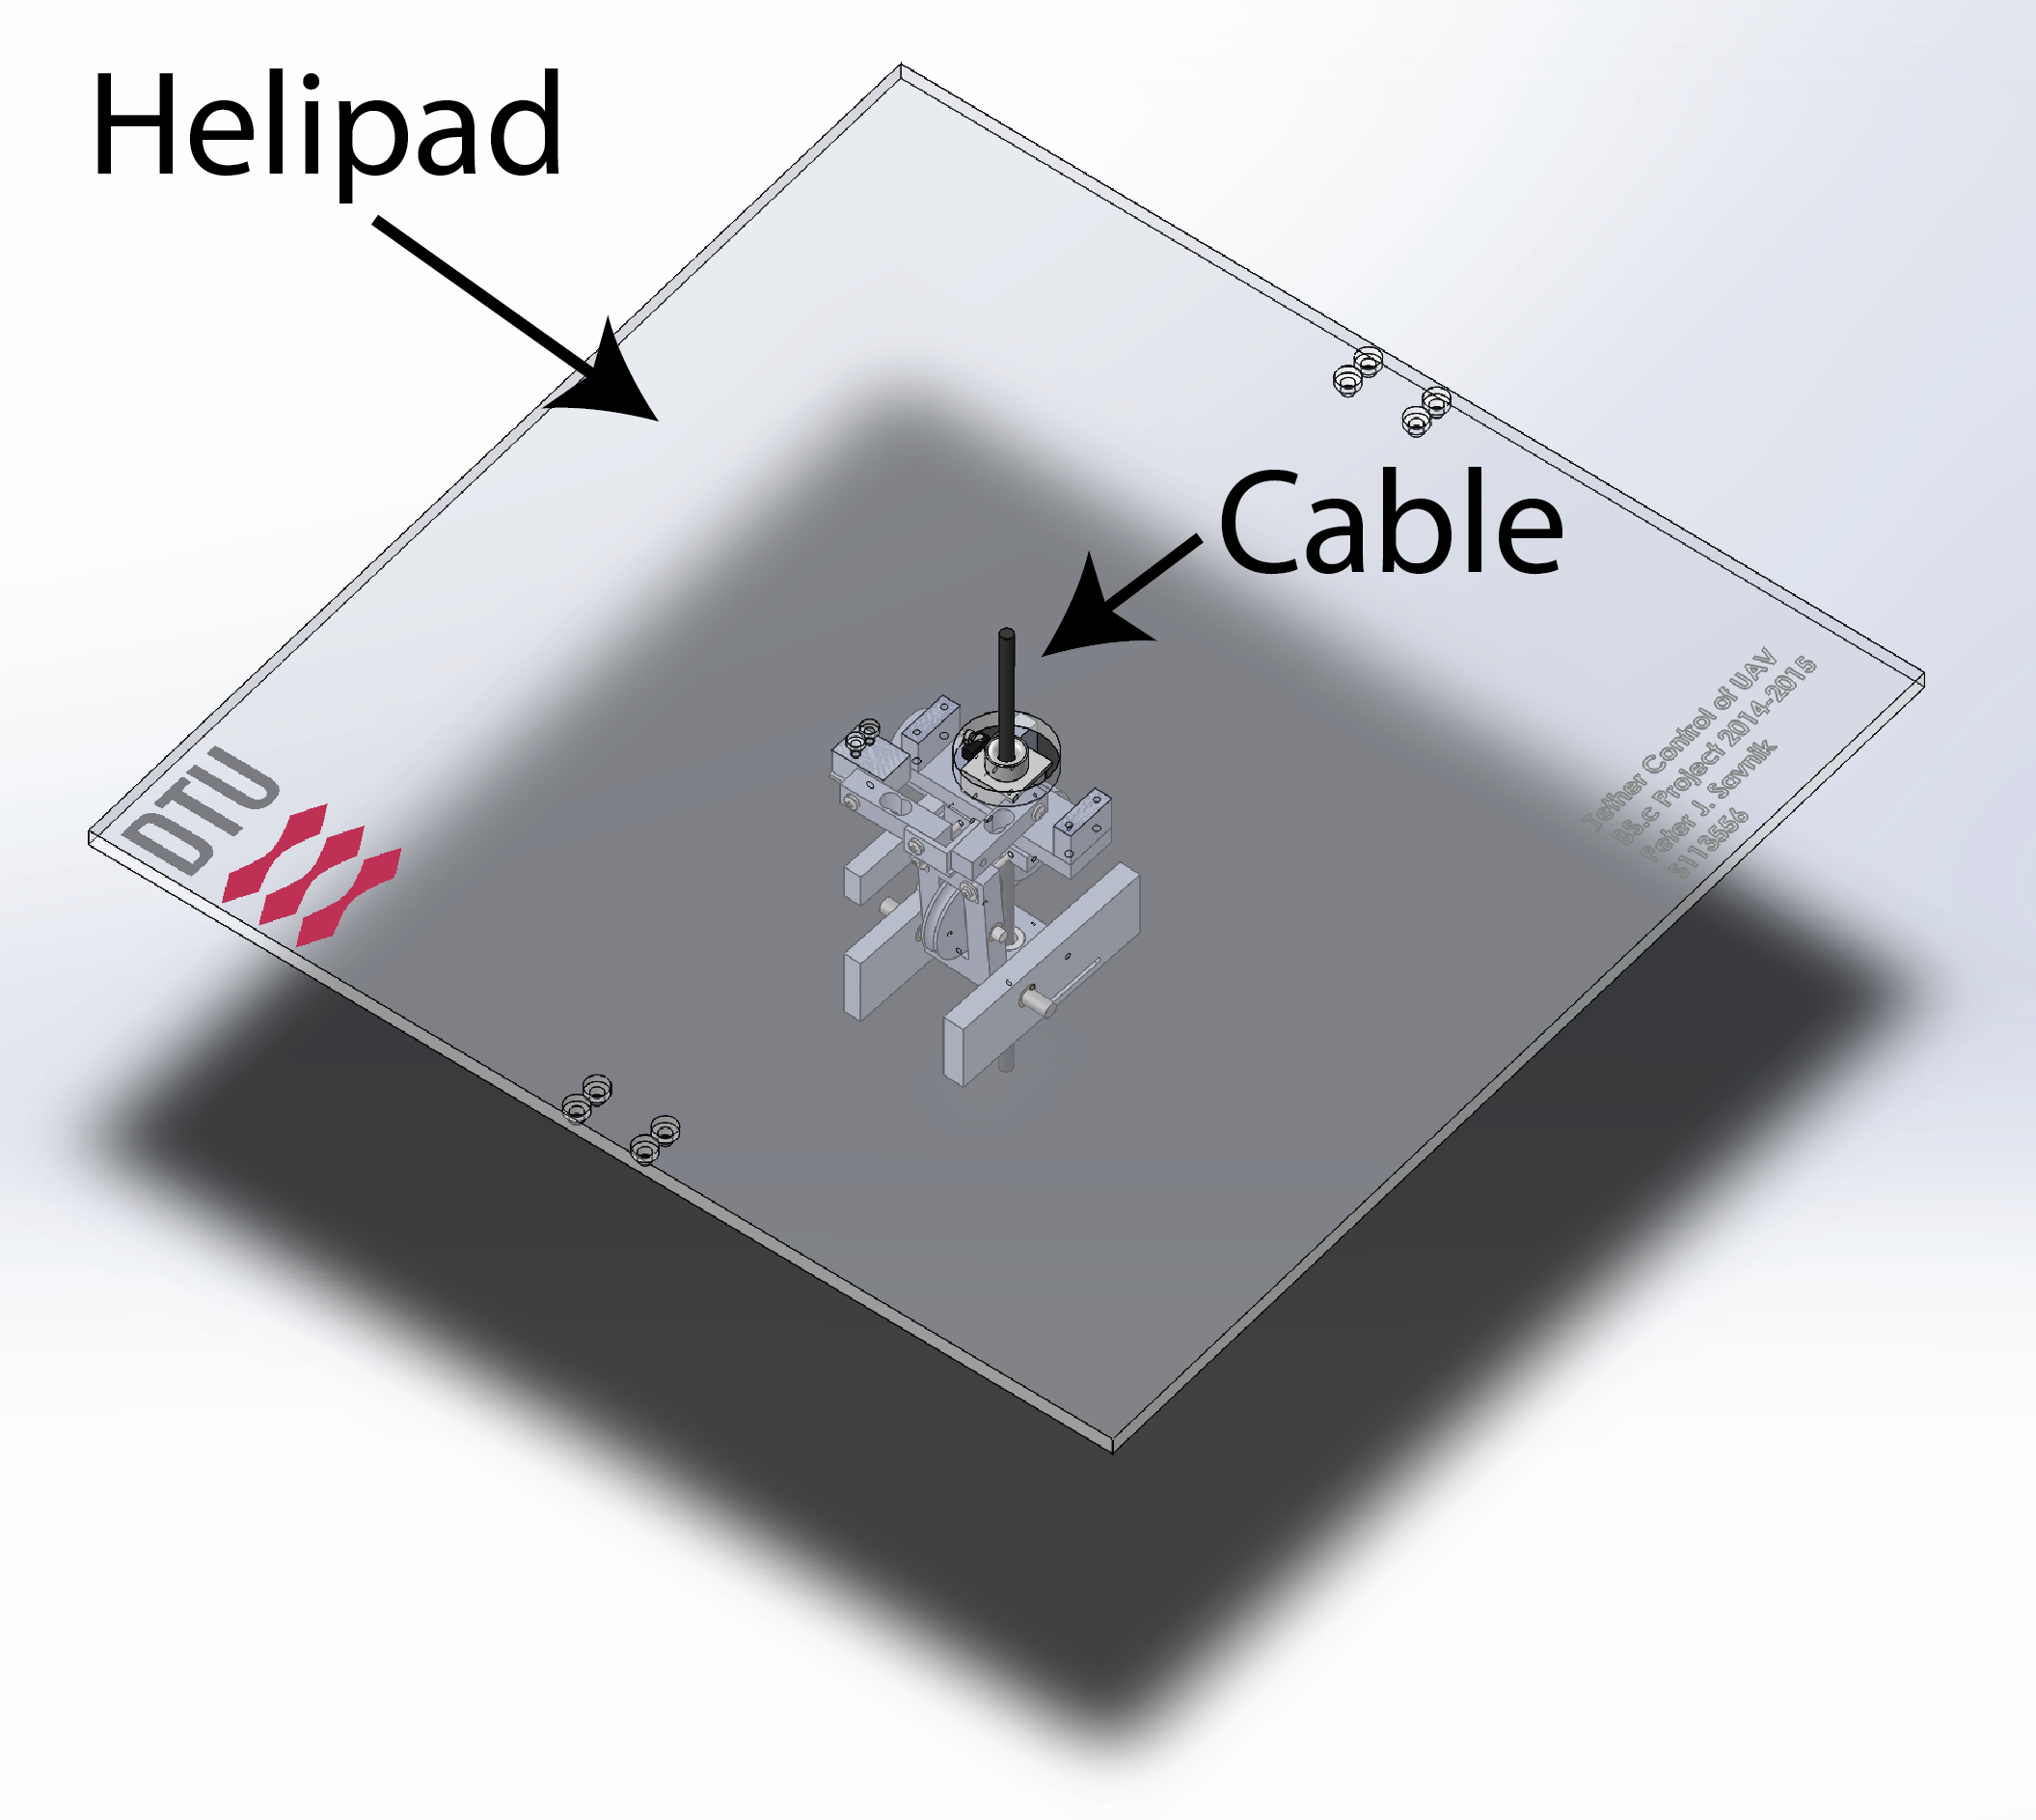
\includegraphics[scale=0.75]{graphics/cad/toplevel.png}
\caption{Illustration of Helipad with a hole in the middle for the cable.}
\label{fig:helipad}
\end{figure}

\section{Messuring the horisontal angle}
\label{sec:horizontalAnglePrototype}
In order to precisely determinate where the UAV is positioned relative to the helipad on a horizontal plane a coordinate system on figure \ref{fig:top-coordinates} is introduced. x and y are cartasian coordinates corresponding to the measurements of loadcell 1 and loadcell 2 from figure \ref{fig:loadcells}. $\phi$ is the angle, starting at the positive x direction and increases in positive direction of rotation.

\begin{figure}[H]
\centering
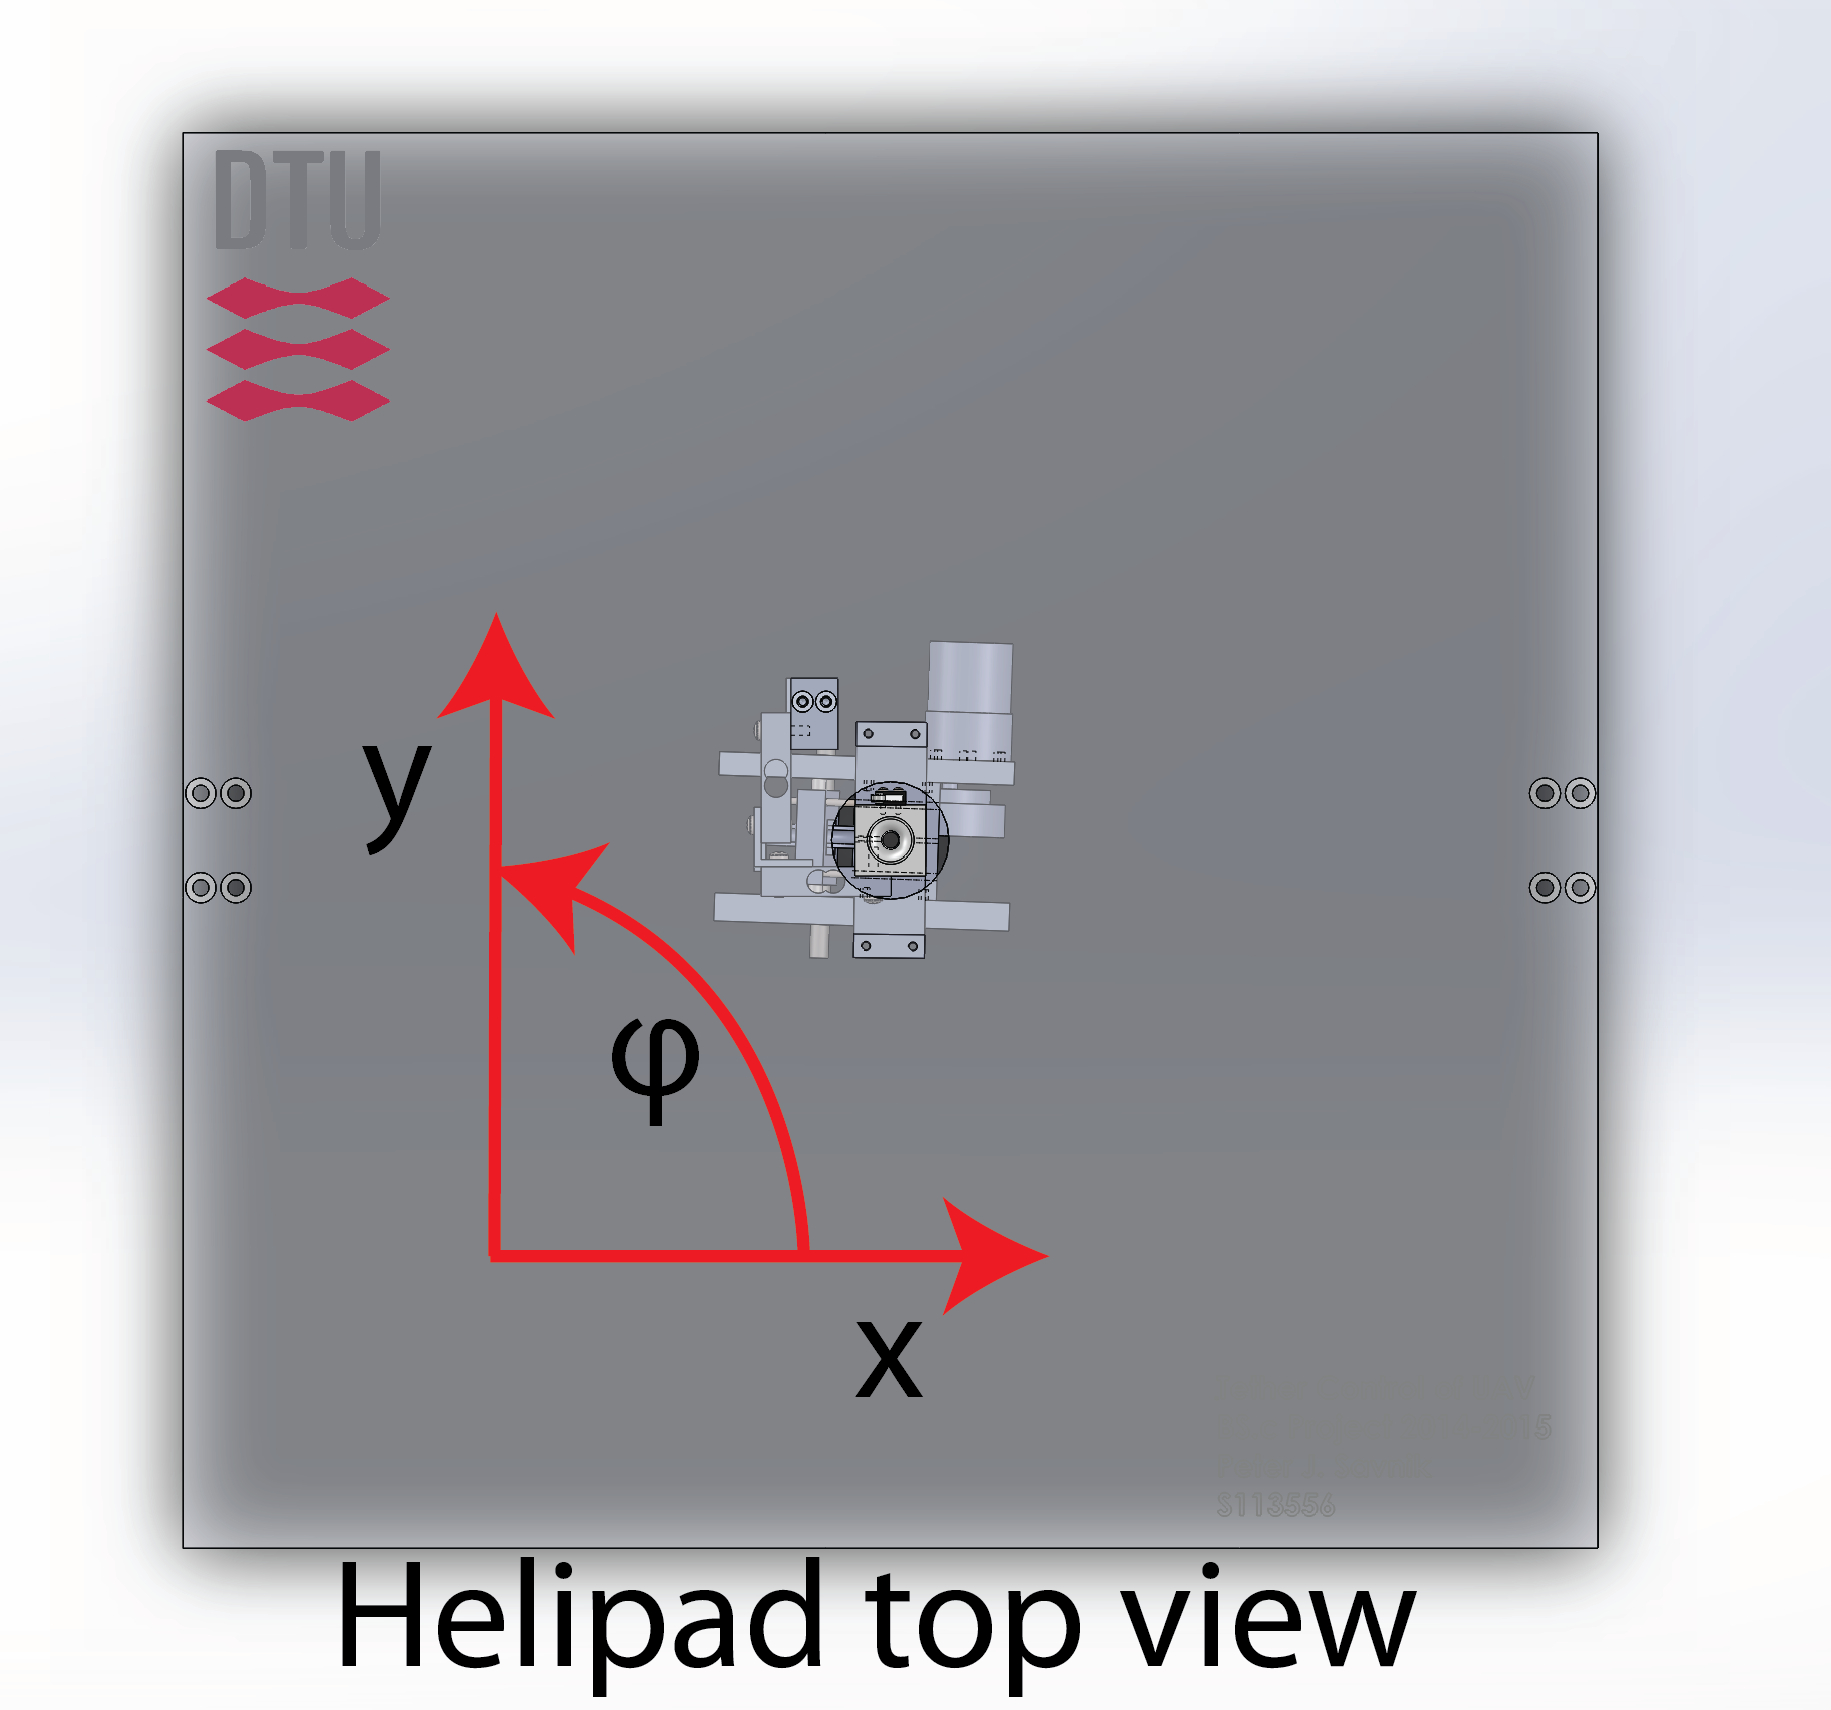
\includegraphics[scale=0.75]{graphics/cad/top-coordinates.png}
\caption{Helipad seen from top view with coordinate system.}
\label{fig:top-coordinates}
\end{figure}

\noindent
To measure the horizontal angle between the ground station and the UAV to loadcells are used, perpendicular to each other. One end attached to the ground station and the other end attached to a cable though hole made in Teflon. Then the UAV is exactly direct over the hole, no force will be measured, but at the UAV moves to one of the sides it will create a cable tension that results in a force in x- and y- direction. Combining the x and y force can be translated to an angle. 

\begin{figure}[H]
\centering
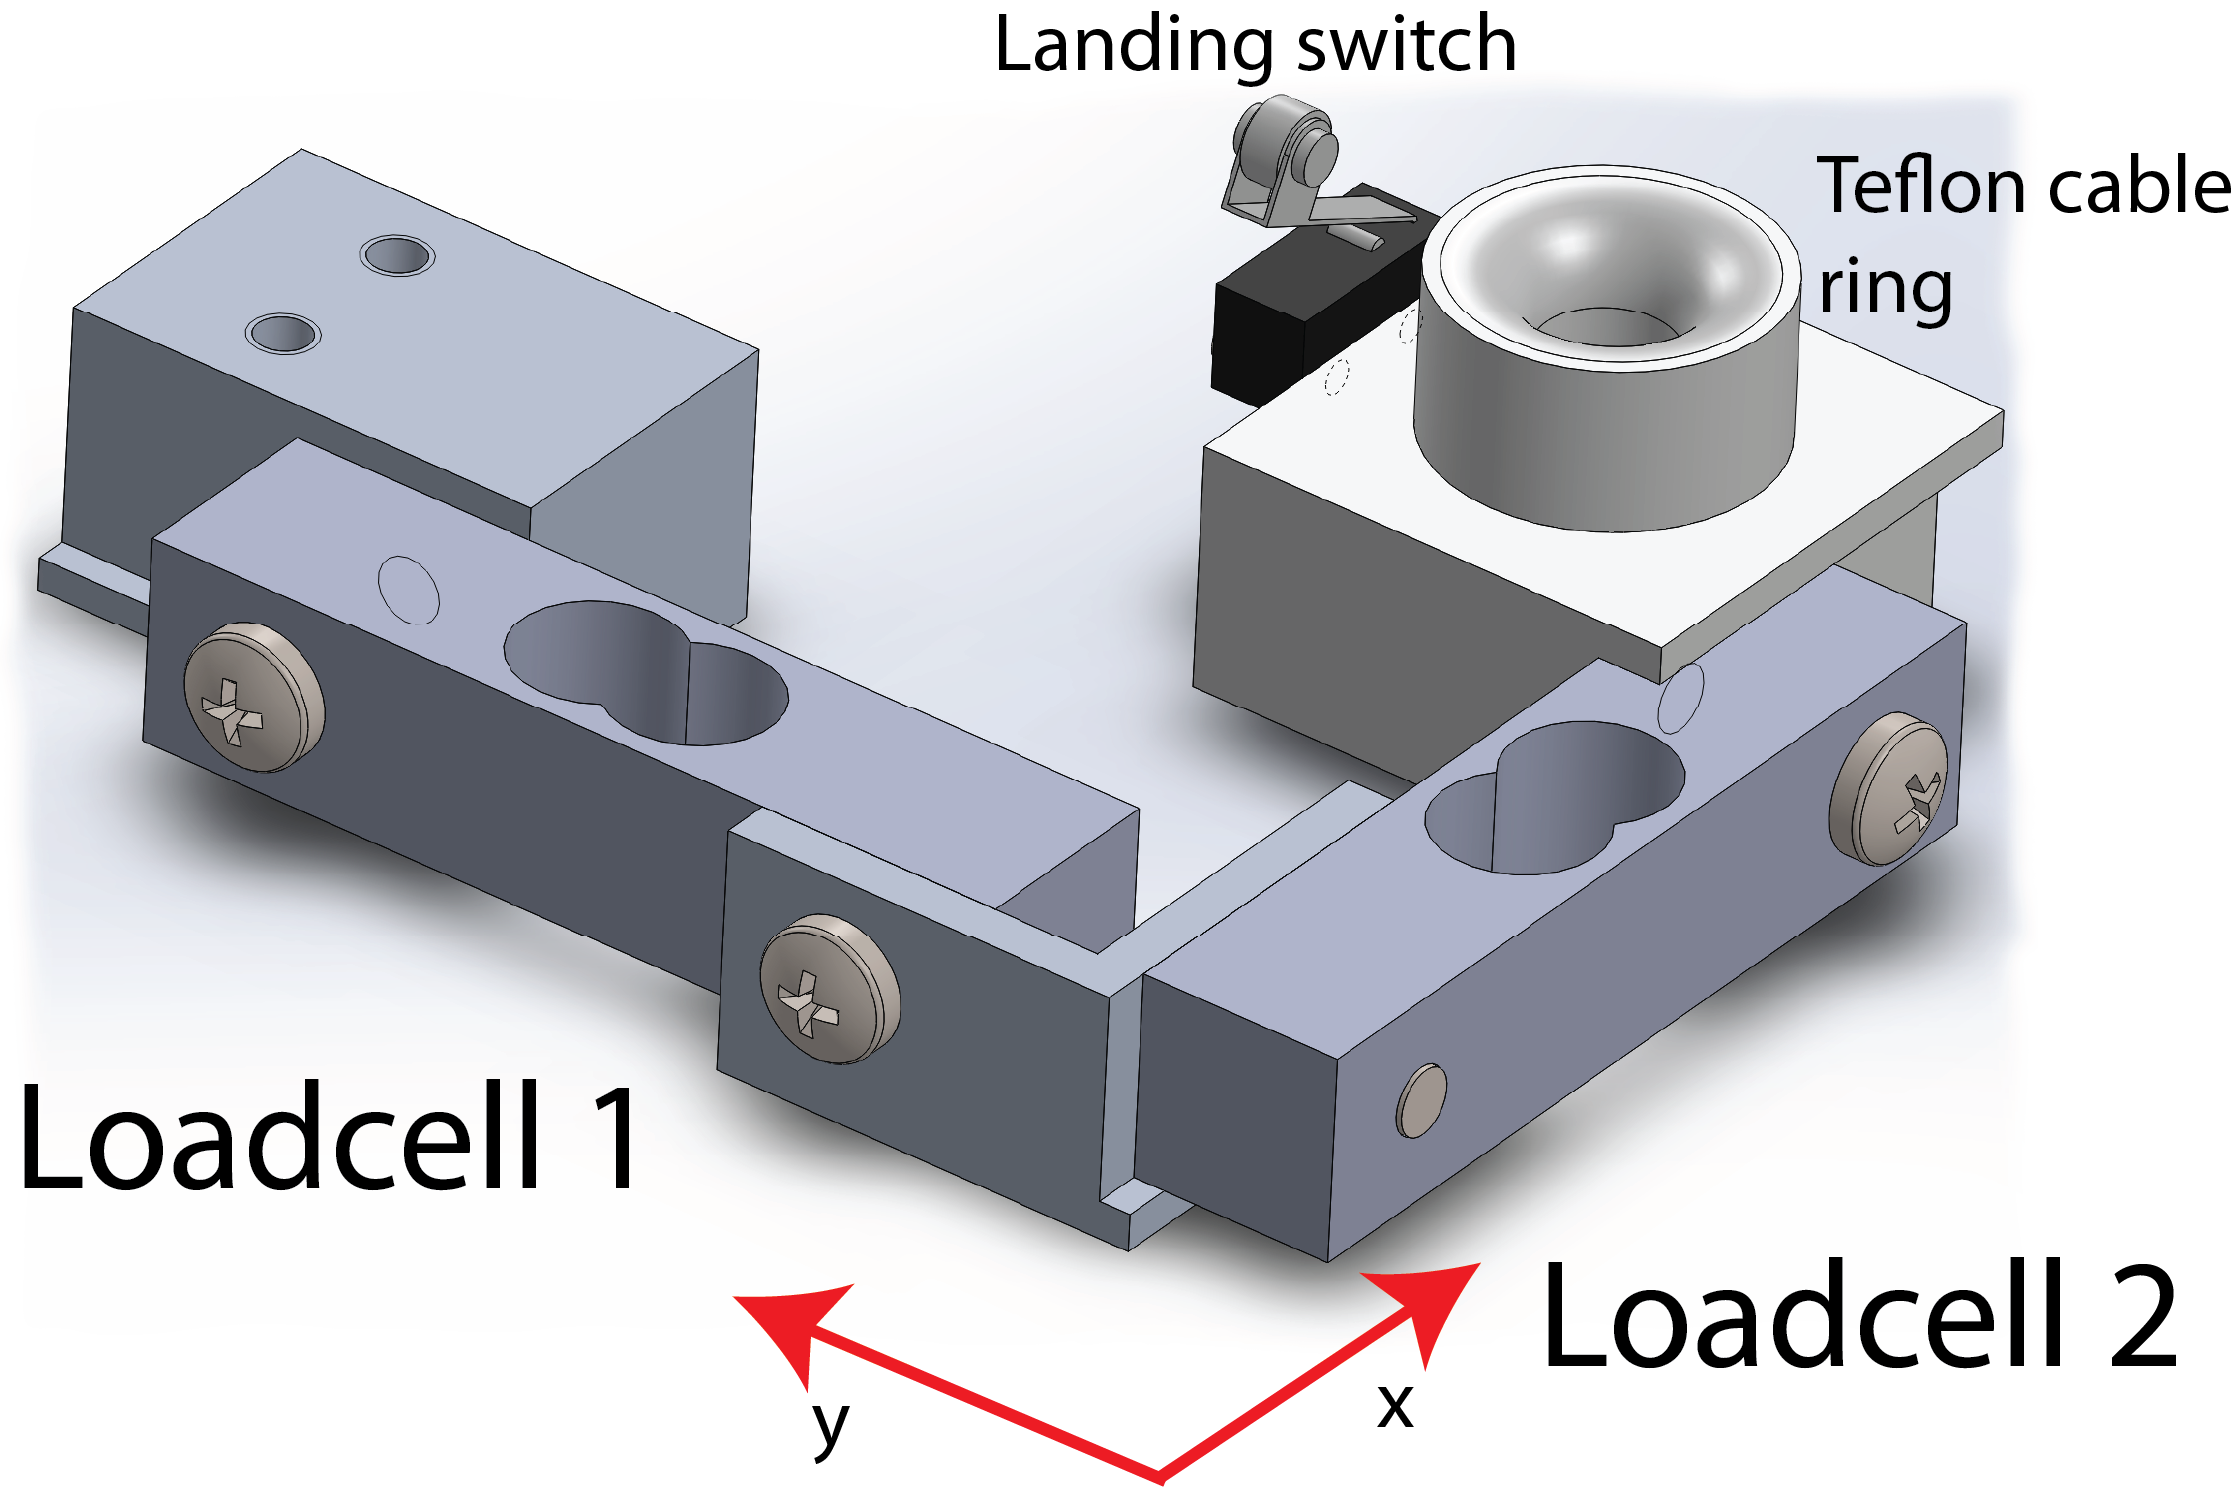
\includegraphics[scale=0.75]{graphics/cad/loadcell.png}
\caption{Configuration of 2 loadcells, for measuring the cable drag in x and y direction. Loadcell 1 measures in x-direction and loadcell 2 in y-direction.}
\label{fig:loadcells}
\end{figure}

\noindent
The UAV can lift about 3kg payload and therefore exert 3kg thrust to the cable and the measuring device must be able to withstand such a force without permanently bending. Two 5kg loadcells from Phidget Inc is assessed to be the best match for the job with regard to what's available in the projects price range.

\subsection{Testing}
First off is calibrating the loadcells. First measurement is without any forces acting in x and y direction in order to determine the offset of each loadcell.
The offset for x is found to $-455.9787$ and the y offset to $-511.2618$.\\

\begin{figure}[H]
\centering
\includegraphics[scale=1]{graphics/gcs_test/calib_0_data_raw.eps}
\caption{Raw input data from loadcell x and y. The average line is the calculated offset used for calibration. Measured without load in any directions.}
\end{figure}

Next 1000g of load is put on the loadcell with a rope through the Teflon ring first purely in positive x direction and next in purely y direction, in order to determine the gain factor $Kx$ and $Ky$. $Kx$ is found to $0.4786$ and $Ky$ to $-0.5134$. Afterwards the calibration is tested by applying $600$g of force in x-direction and then checking the result.

\begin{figure}[H]
\centering
\includegraphics[scale=1]{graphics/gcs_test/calib_result_compare.eps}
\caption{Comparing raw data to the calibrated values. The x-calibrated values are between $633$g and $636$g, then the force applied was $600$g. The $33-36$g difference is most likely caused by the limitations of precision from the spring load. The y-calibrated data is ranging from $-29$g to $-32$g. It is expected the precision can vary $\pm75$g around the zero balance.}
\end{figure}

\noindent
Second test is done by applying a known force in a combination of x and y direction. For this test $\phi$ is set to 45 degrees and the total force is $1$kg. On figure \ref{fig:phi45deg1kg} it is seen that the data slightly decreases over time. This is probably due to tolerances in the manufacturing process enabling the loadcell to move slightly over time.

\begin{figure}[H]
\centering
\includegraphics[scale=1]{graphics/gcs_test/phi45deg1kg.eps}
\caption{This test combines both x and y direction, therefore the force is calculated into the variable $r$, equivalent to $T_0$ from the analysis chapter. Notating at around $1$kg of load the data drift slightly towards 0.}
\label{fig:phi45deg1kg}
\end{figure}

\noindent
On figure \ref{fig:phi45deg1kg} it is seen that the data slightly decreases overtime. This is probably due to tolerances in the manufacturing process enabling the loadcell to move slightly over time or it can be caused by the spring load is permanently bending. Taking a closer look at the data on figure \ref{fig:phi45deg1kgdata} showing this phenomena applies to both x and y loadcell. Because it applies to both loadcells the calculated angle $\phi$ is constant, thus the drift the data is still valid and results in an accurate angle.

\begin{figure}[H]
\centering
\includegraphics[scale=1]{graphics/gcs_test/phi45deg1kgdata.eps}
\caption{Showing the calibrated data from x and y loadcell then 1kg of load is applied with $\phi=45$ degrees.}
\label{fig:phi45deg1kgdata}
\end{figure}



\noindent
Second test was done keeping the $\phi$ angle and the tension constant and varying the $\theta$ angle. Is is expected as $\theta$ approach $90$ degrees the measured force will be approaching $0$. 
\begin{figure}[H]
\centering
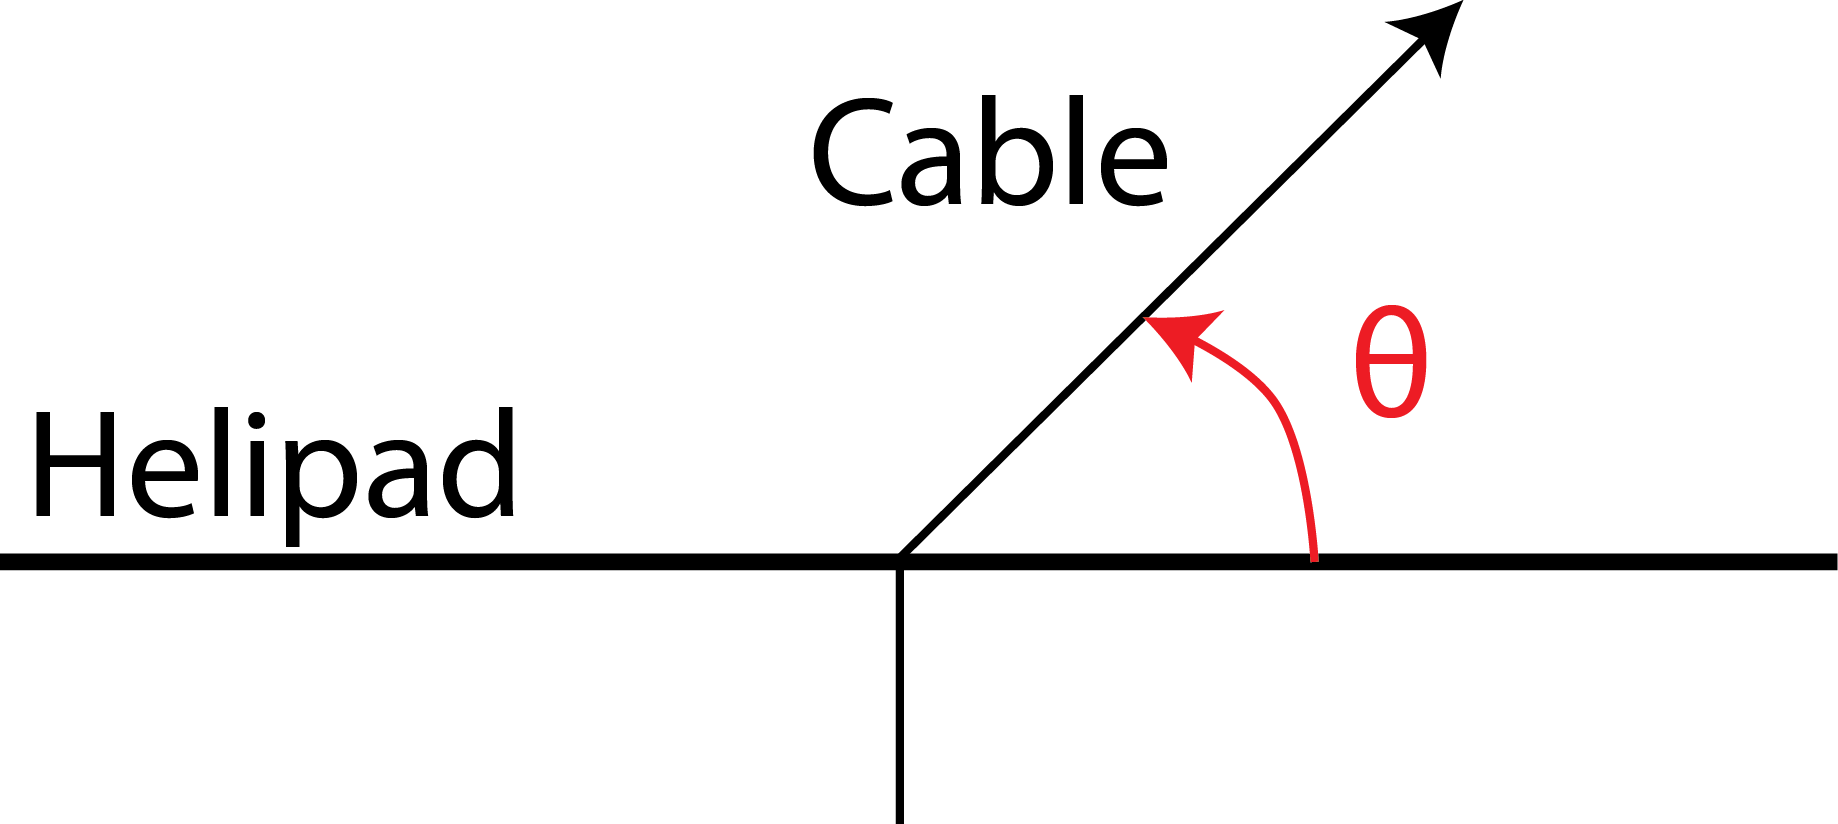
\includegraphics[scale=0.75]{graphics/loadcell_test2.png}
\caption{Testing the horizontal measuring device by keeping $\phi$ constant and varying $\theta$.}
\label{fig:loadcell_test2}
\end{figure}

At $\theta=45$ degrees and 1kg of load the measured result is very close to the expected result.

\begin{figure}[H]
\centering
\includegraphics[scale=0.75]{graphics/gcs_test/45degTheta1kg.eps}
\caption{Comparing the measured load to the theoretical value. Showing slightly less than expected.}
\label{fig:45degTheta1kg}
\end{figure}

\noindent
At all previous tests the load has only been anchored in the Teflon ring, but in the real setup the cable are anchored in the winch instead. This mean the measured force is now only a component of the total force. From figure \ref{fig:catenary_force_diagram} $T_0$ only has an x-component, but when the cable now is anchored in the winch the total force equation change to
\begin{equation}
\sum T -\lambda gs + (T_{0,x} + T_{whinch,y} ) = 0
\end{equation}
Hence the measurement device only measures $T_{0,x}$, $T_{whinch,y}$ is unknown. This test will show how much $T_{winch,y}$ influences.
On figure \ref{fig:45degTheta1kg} the measured values are slightly higher than expected. At $\theta = 0$ the overshoot is $13-17$g and at $\theta = 45$ the overshoot is $28-32$g, which is within what's in the first test was discussed as due to limitation in precision. 

\begin{figure}[H]
\centering
\includegraphics[scale=1]{graphics/gcs_test/Theta1kgCable.eps}
\caption{Comparing measured results to the theoretically expected when varying $\theta$ and 1kg load. The results is a little higher than expected, but comparing to figure \ref{fig:45degTheta1kg} this result is unexpected.}
\end{figure}




\subsection{Summary}
The prototype is able to measure the force in x- and y-direction, $\phi$ and $r$ can be calculated with good results. Higher precision might be possible with more precise testing equipment.
The 5kg loadcell has a zero balance at $\pm75g$. Any values close to this range must be considered as very unreliable. 
The force in $T_{winch,y}$ is quite small and can therefore be ignored.




\section{Winching and storing the cable}
There are several ways to keep the cable when it's not rolled out, 2 commonly used methods are on a cable drum or in a winded pile. The critical parameters here is the flexibility of the cable, diameter of the cable and heat tolerances.  Because the cable is stored tightly together, heating from the cable resistance has to be given a thought in the cable storing design.

\subsection{Storing cable on a drum}
Storing cable on a drum is a very practical and commonly known method to store cables in a organised way. The benefits of this design is that the drum it self can be used as a winch to winch in the cable. But the minimum diameter of the drum is given by the cable minimum bending radius for flexible installation and that sets a physical minimum for the drums outer diameter. The larger the diameter the greater the force needed for rotating the drum. To assure smooth windings the drum can move from side to side. Due to physics the movement from side to side will come natural, if the friction is low enough; in practise this concept works often but is not robust and that is why motorized guidance is needed\todo{referance}. In theory the rotation of the drum can be used as a feedback for how much cable is rolled out, but in practice this will be a source to a large margin of error. Further more this design is very dependent on the cable all ways has tension. If there is no or too little tension on the cable it will loosen from the drum. \\
On figure \ref{fig:cable-drum} a cable drum is put under the helipad and the horizontal measurement device. 

\begin{figure}[H]
\centering
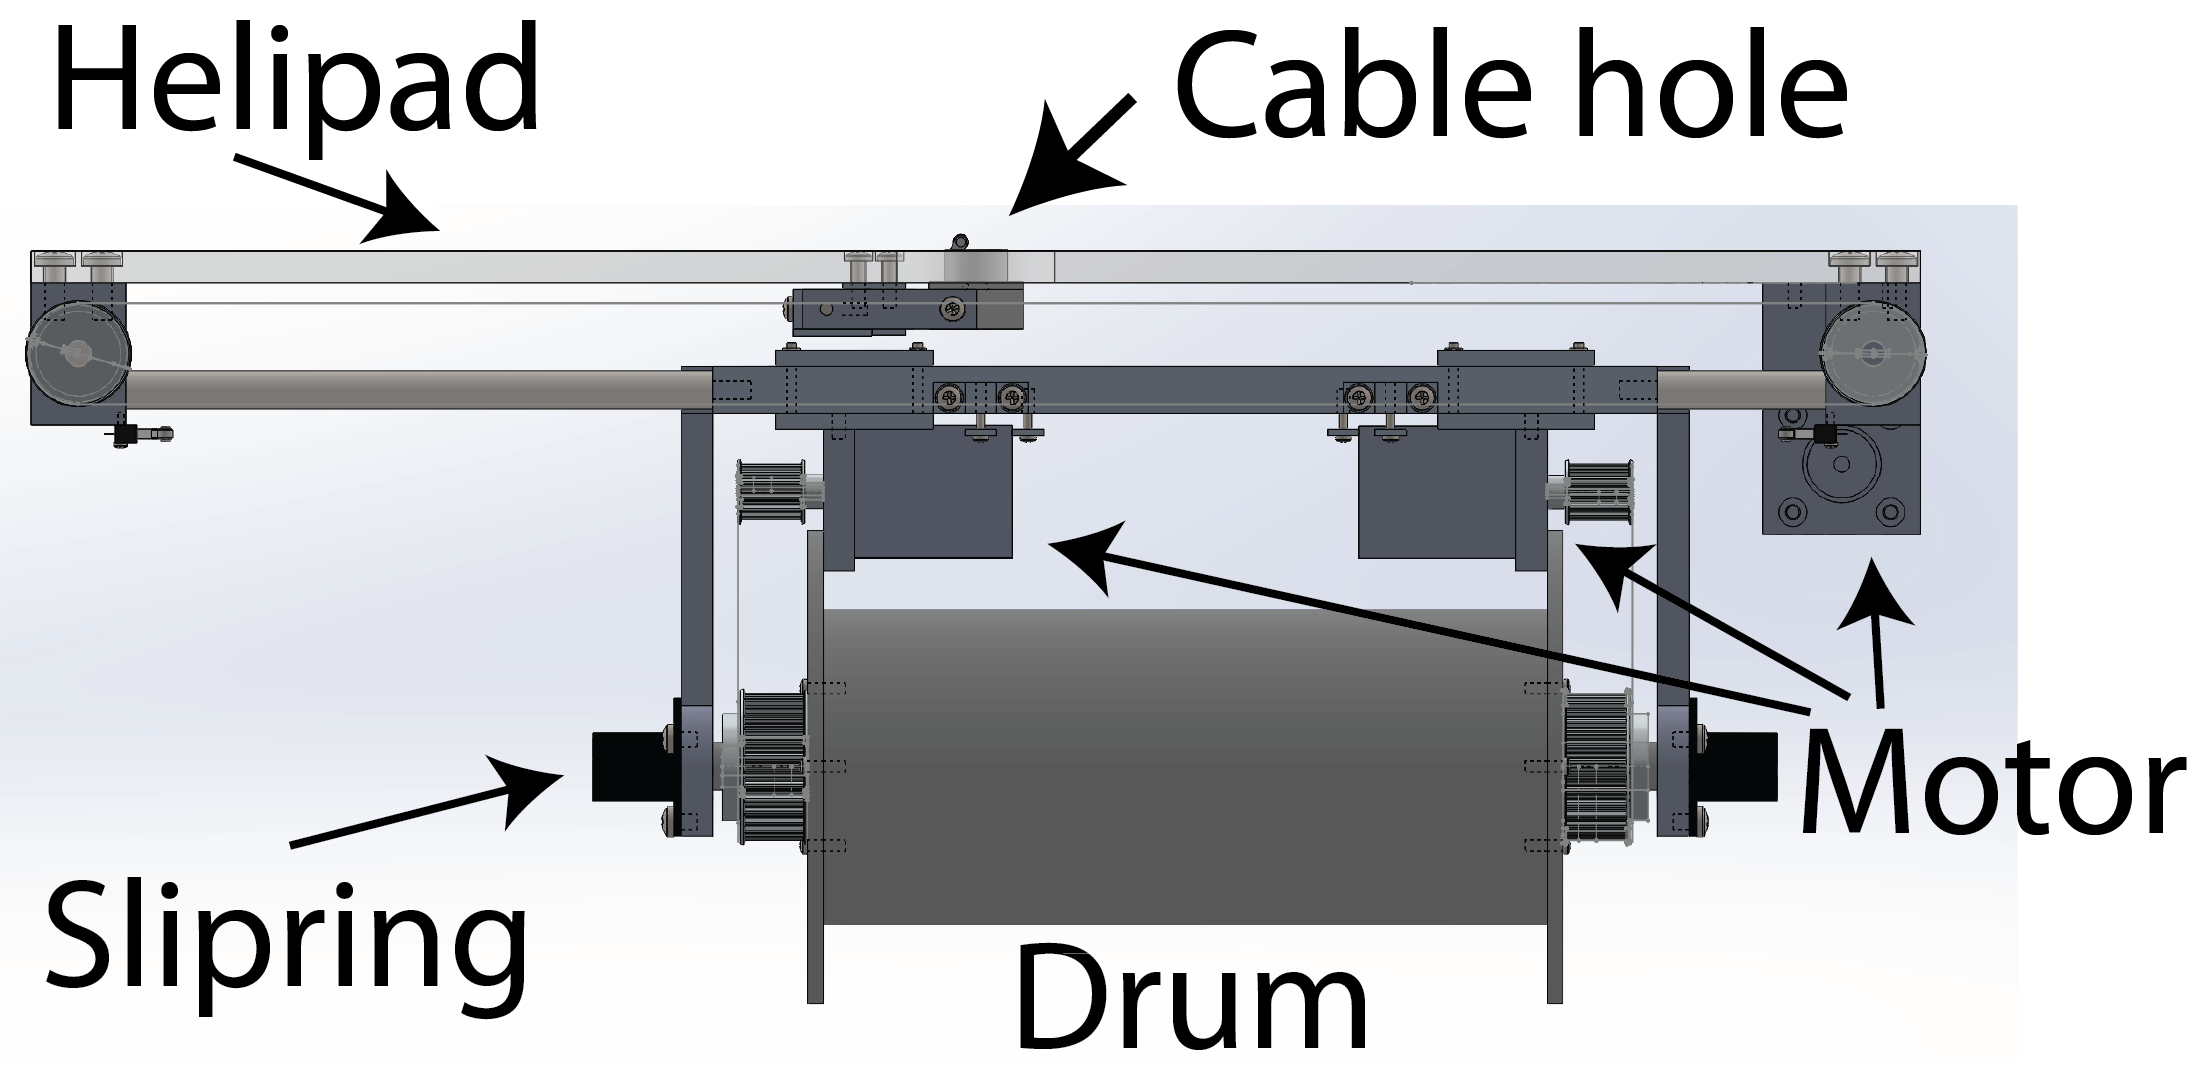
\includegraphics[scale=0.75]{graphics/cad/cable-drum.png}
\caption{Cable drum design. The drum can rotate to winch in/out the cable, and also move from side-to-side to assure smooth windings.}
\label{fig:cable-drum}
\end{figure}

\noindent
With all wire winded in and the UAV on maximum throttle there is assumed to be 500W running through the cable with a electrical loss of around 120 Watt, which is transformed into heat. 120 Watt of heat will give rise to heating up the cable drum. This is a known cause of electrical fire, when a cable drum gets too hot and melts. Therefore a series of pretests where performed to address how big a problem this would bee and too incorporate the result in the design of the system. 

\noindent
The worst-case test with full load over long time was performed at indoor environment with room temperature on 24 degree Celsius. The coil was excited with 75V DC and 30A just over an hour. The inner diameter of the coil is 10cm and is made of 2mm thick PVC pipe.
\todo{Skelne tydligere mellem 75 volt siden og 12 volt siden}

\begin{figure}[H]
   \centering
   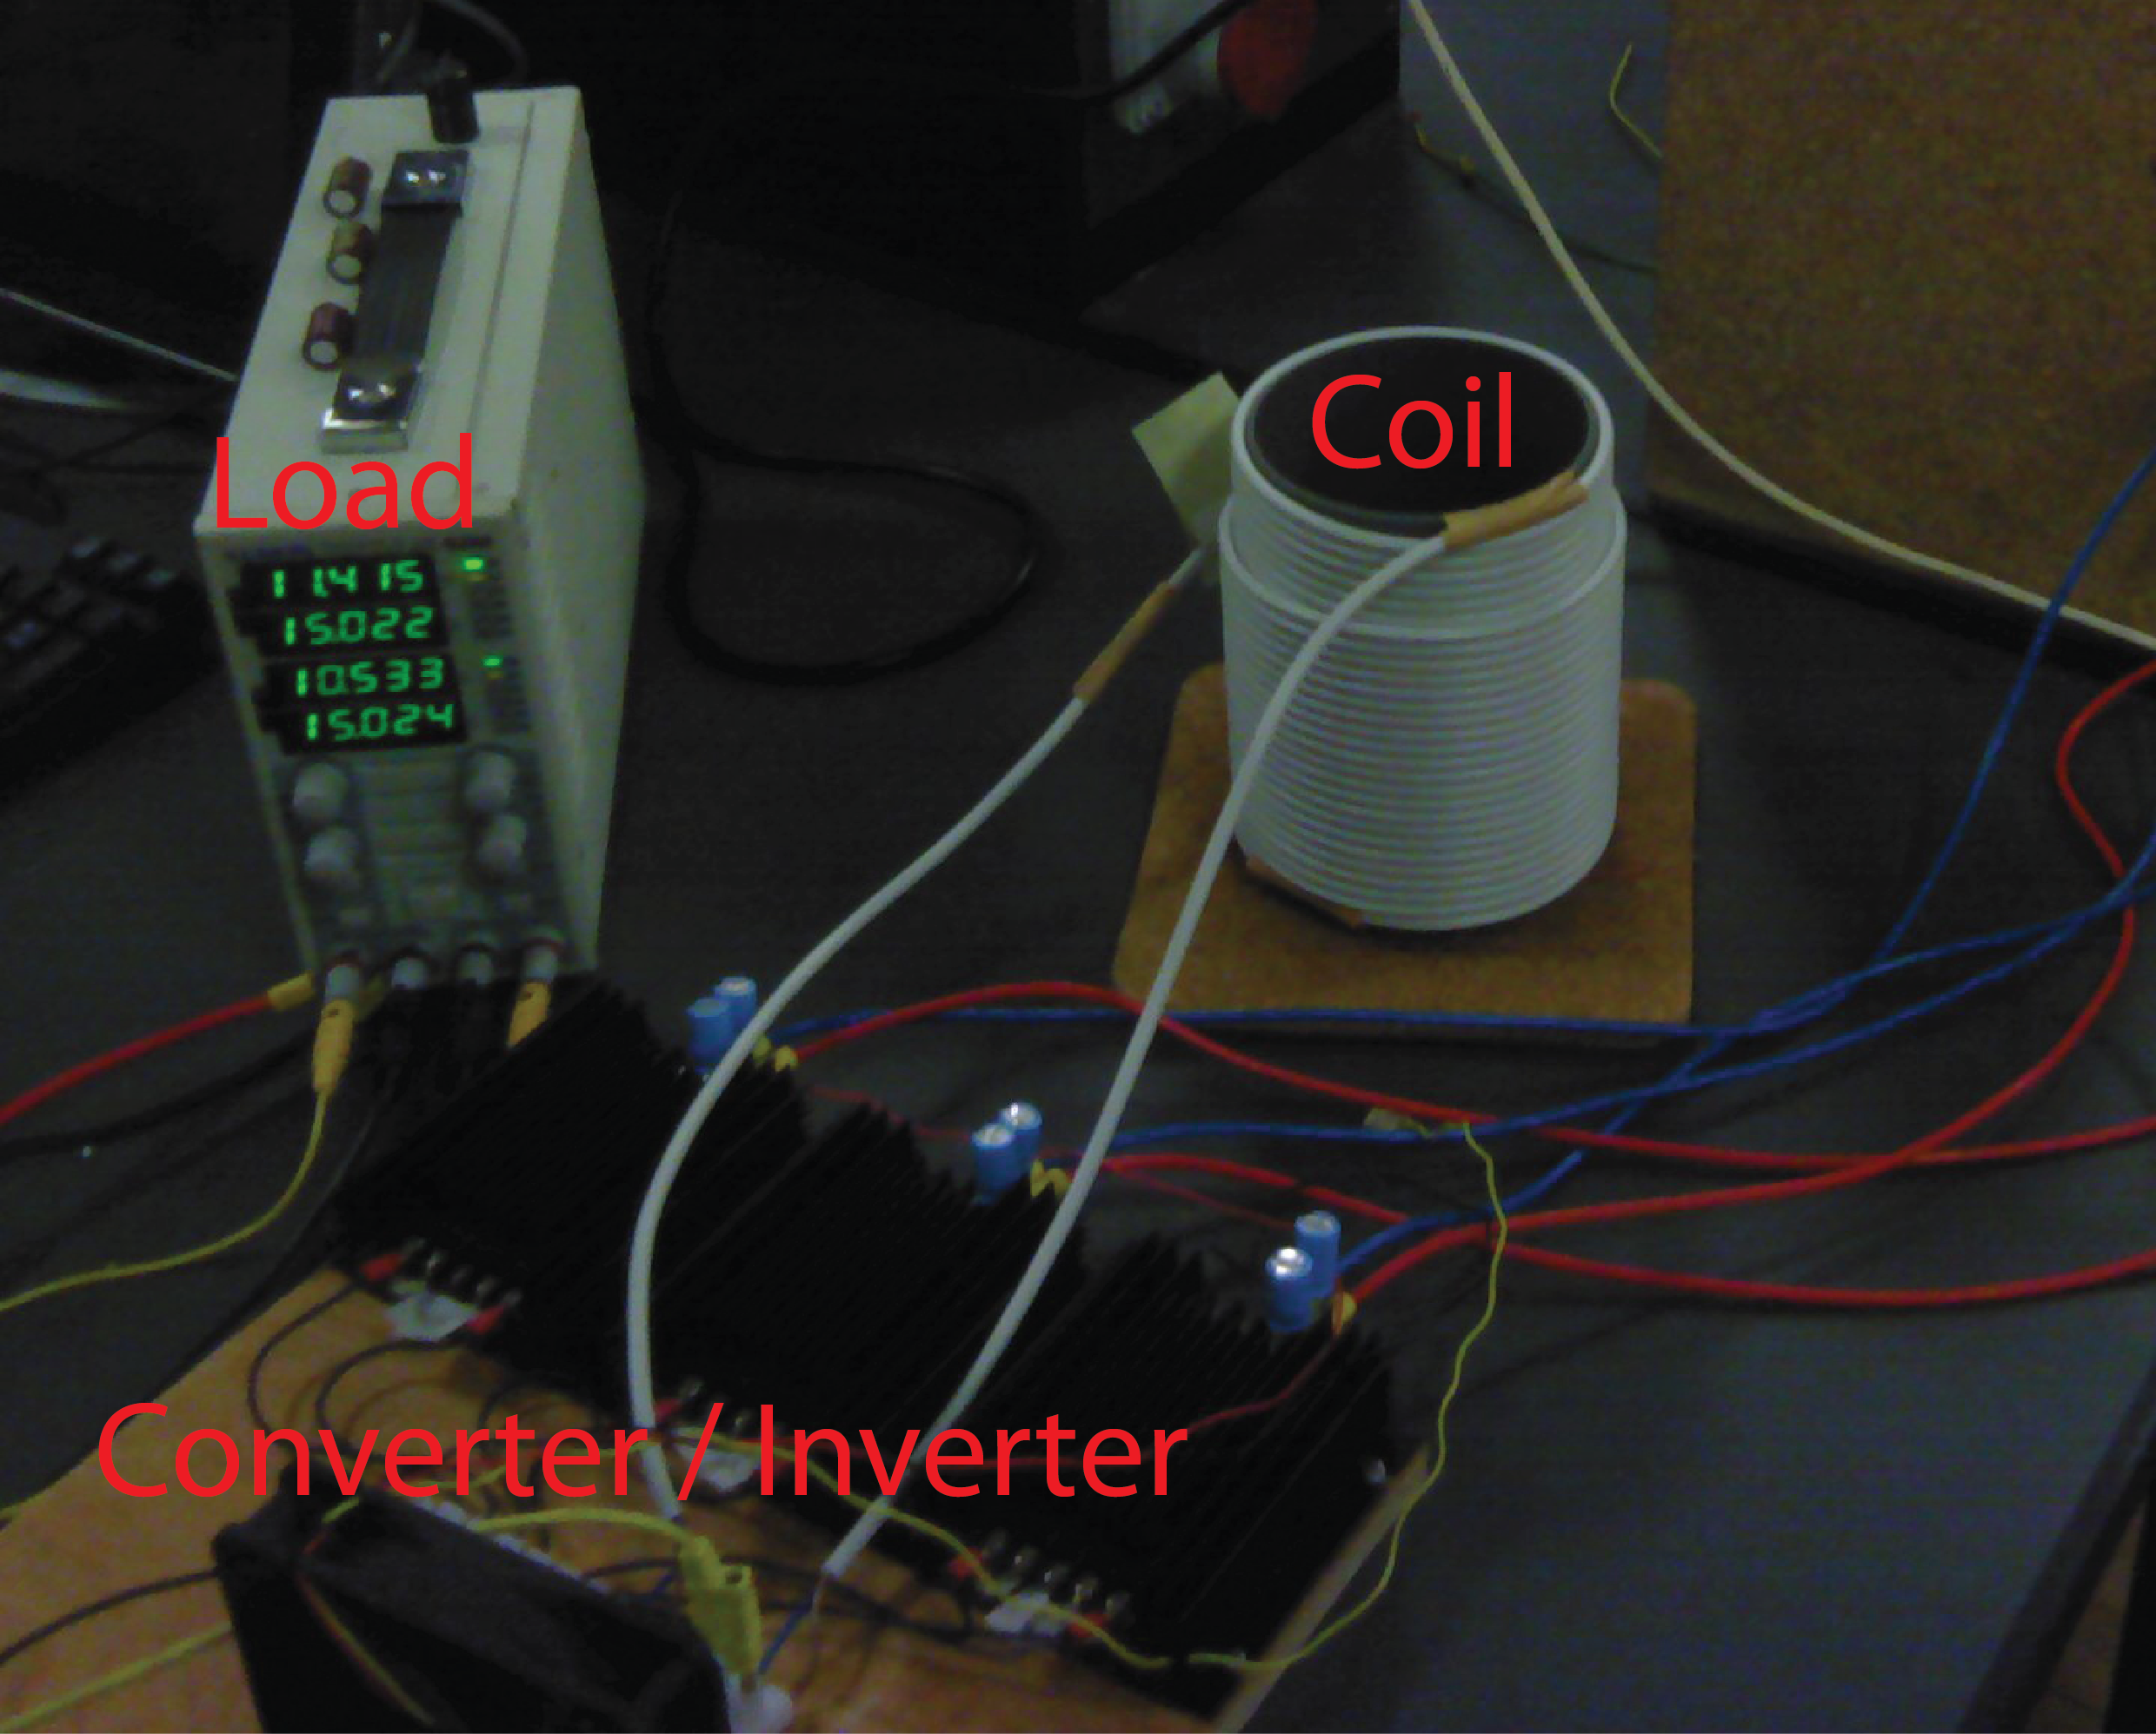
\includegraphics[scale=0.5]{graphics/heat_test/heat_test_setup.png}
   \caption{Heat test setup showing the coil, the test load and power Converters.}
   \end{figure}
      

\begin{figure}[H]
\centering
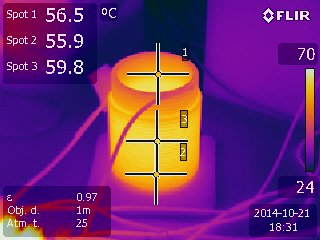
\includegraphics[scale=1]{graphics/heat_test/IR_1491.jpg}
\caption[Caption for LOF]{Heat test of 20m standard household cable\footnotemark winded in 2 layers with 75V DC and 30A. Spot 1 is inside the coil, spot 2 is the lower side of the outer coil and spot 3 i at center of the outer coil. On the lower left corner thermometer calibration constants is displayed.}
\label{fig:heat_test_ir}
\end{figure}
\footnotetext{House hold cable with unknown origin, cross-sectional area 0.75mm2, Max voltage 230 AC, Max current 10A}

\todo{Lav matlab plot af data}

\subsection{The Simple Winch}
Sometimes simple is better. The simple design has a motorized toothed wheel and an encoder wheel pushing the cable against the motorized wheel. The encoder wheel turns only when the cable is moving, and the slip is minimal making it a very robust feedback for the motor controller. The encoder wheel is pushing the cable toward the motor wheel with a spring, that assures small imperfections in the cable does not make it slip. two simple screws adjust the spring tension. For storing the cable a box underneath collects the cable.

\begin{figure}[H]
\centering
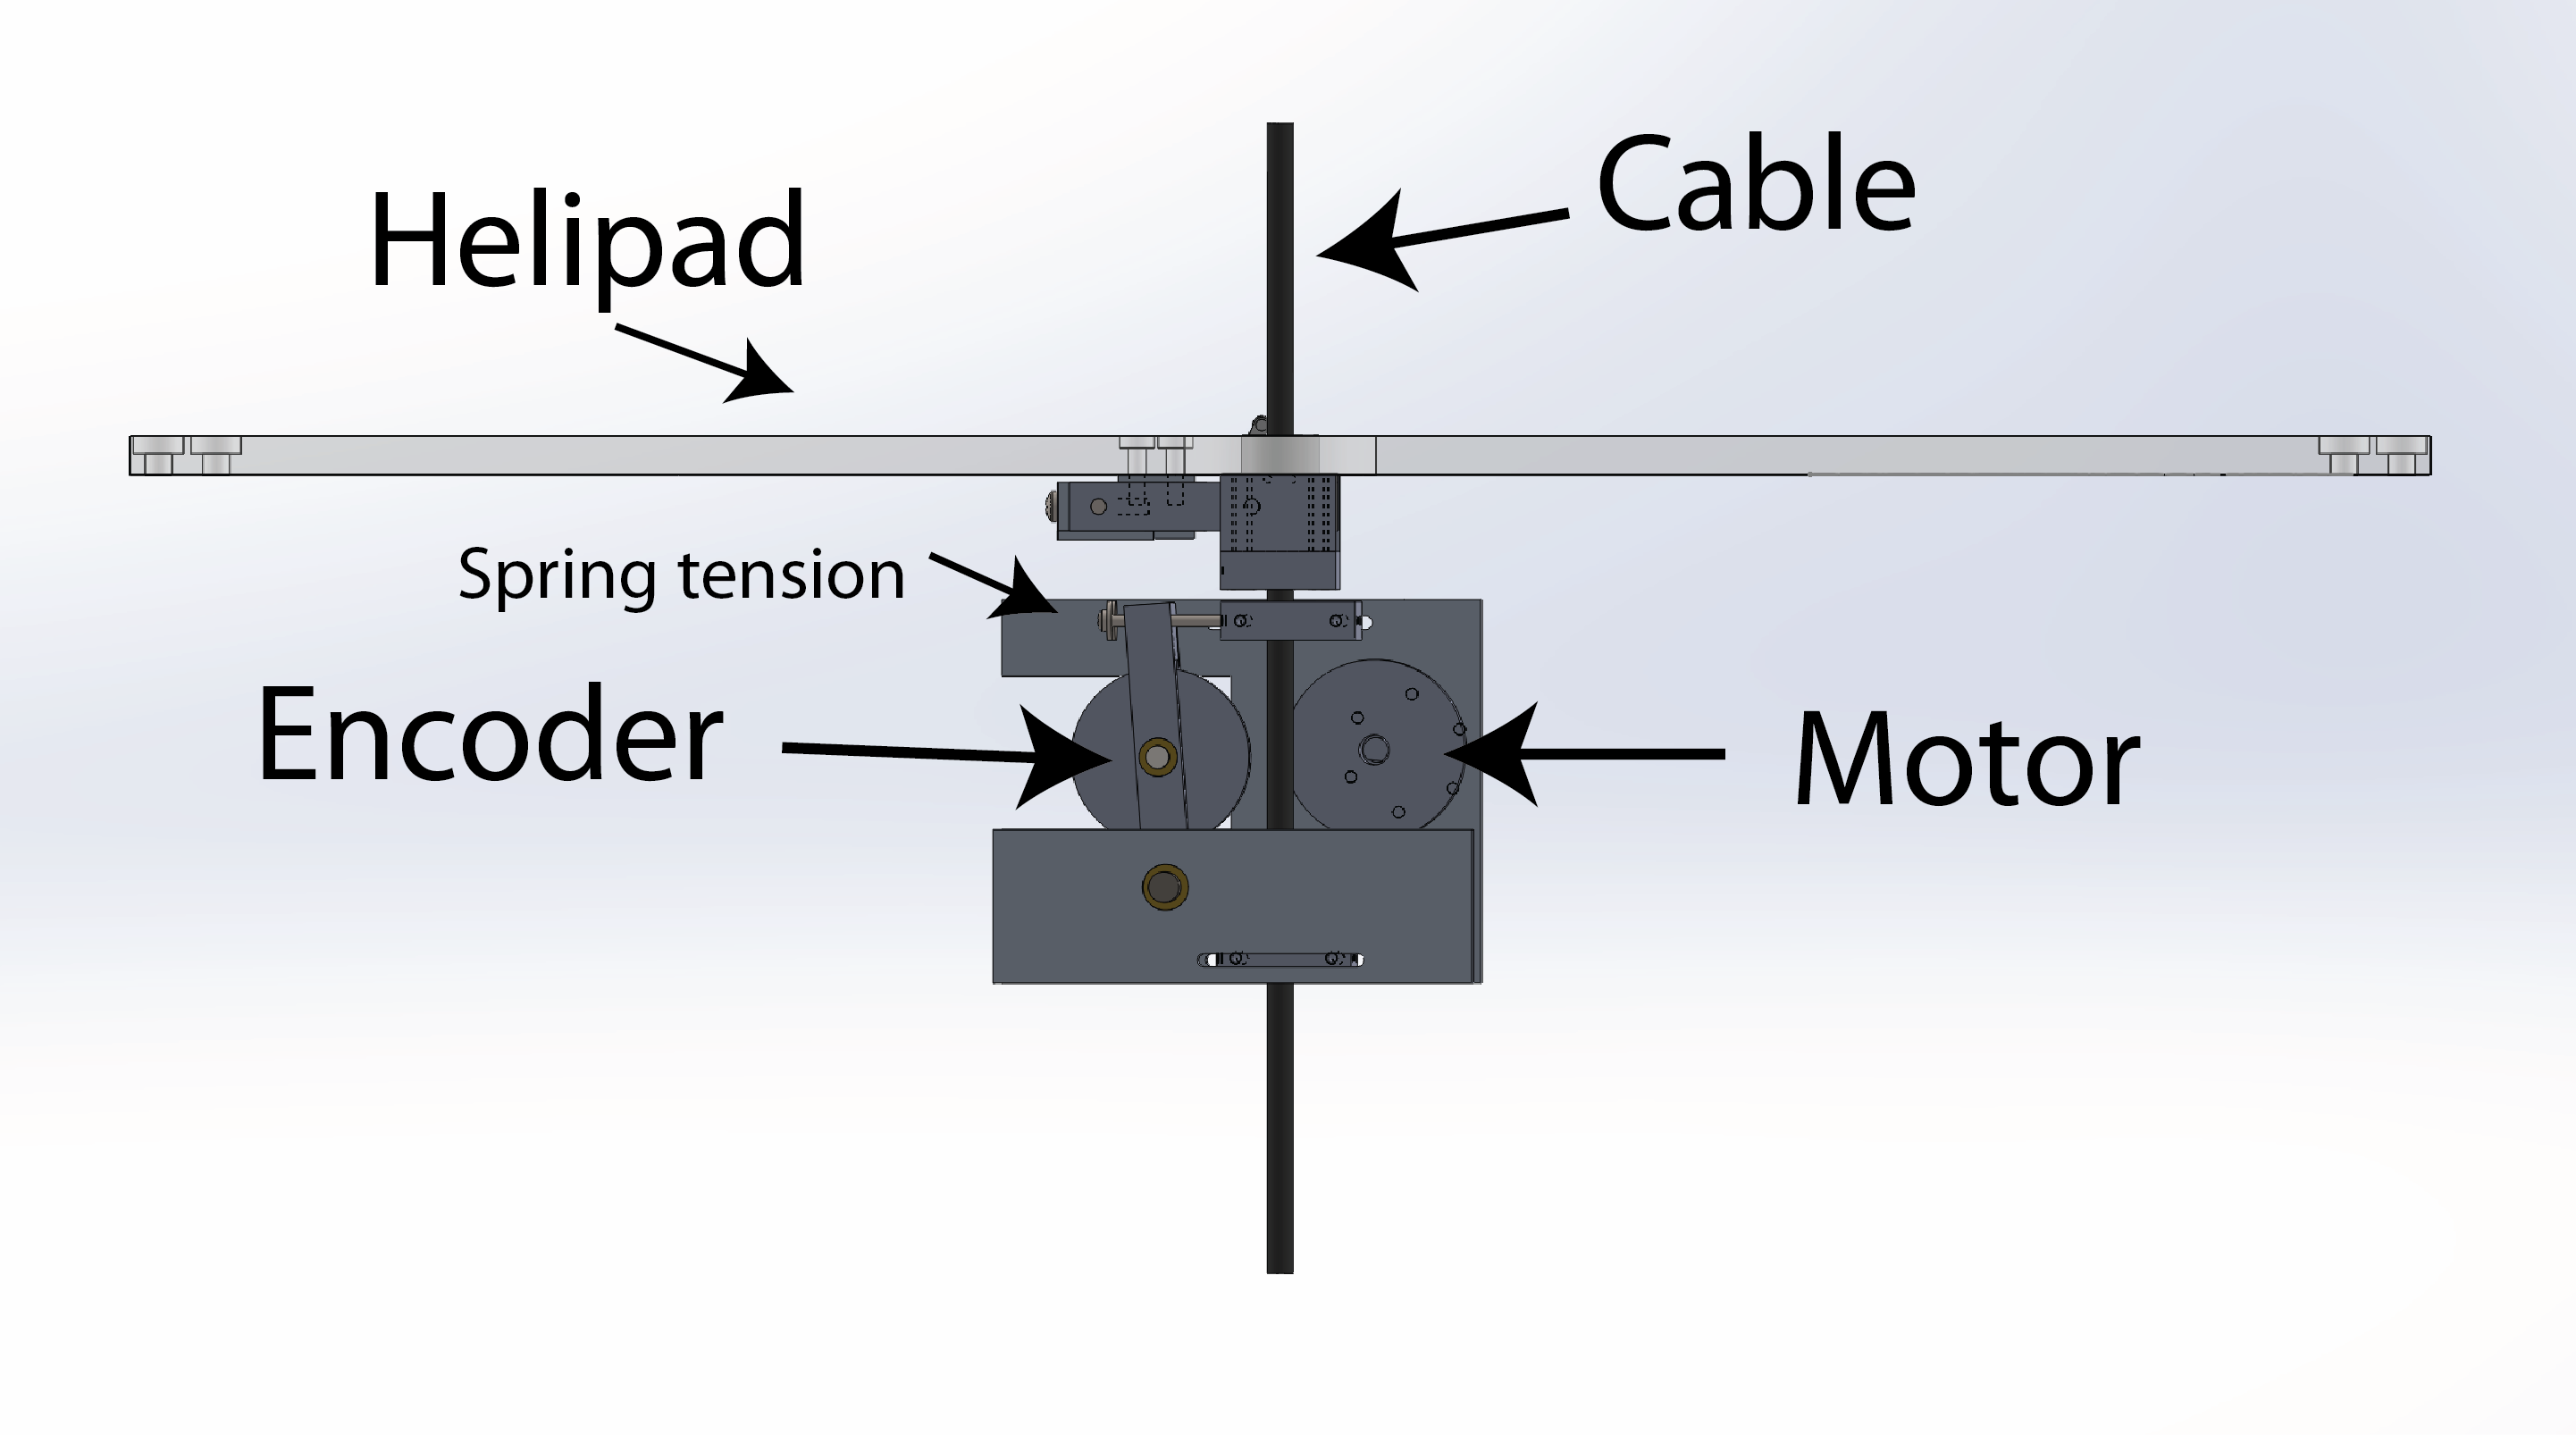
\includegraphics[scale=0.75]{graphics/cad/winch.png}
\caption{The Simple Winch only has one motor and an encoder wheel pushing the cable towards the motor wheel. Two springs adjust the tension.}
\label{fig:winch}
\end{figure}

\subsection{Summary}
Both concepts are mature enough to be prototyped and tested, but due to the time frame of this work there is only time for manufacturing and testing one design. Based on the lower mechanical complexity of the simple winch, the simple winch is the chosen design.    


\section{Cable Connection point on the UAV}
Connecting the cable to the UAV have several issues to address. First a 3-axis measurement device is needed to measure how much the cable tension is and in tree directions - x, y, and z directions. The loadcells used is of same type as in measuring the horizontal angle in section \ref{sec:horizontalAnglePrototype} on page \pageref{sec:horizontalAnglePrototype}. In z-direction the maximal force applied to the loadcell is the UAVs lifting capability on approximately 3kg\todo{Citer adriana}. Hence the choise of loadcell is a 5kg loadcell.\\
\noindent
In x- and y-direction the force applied by the cable or the UAV is not expected to exceed $0.5$kg, thus two smaller $0.78$kg loadcell is used to measure the x- and y-directional force. 

\begin{figure}[hbtp]
\centering
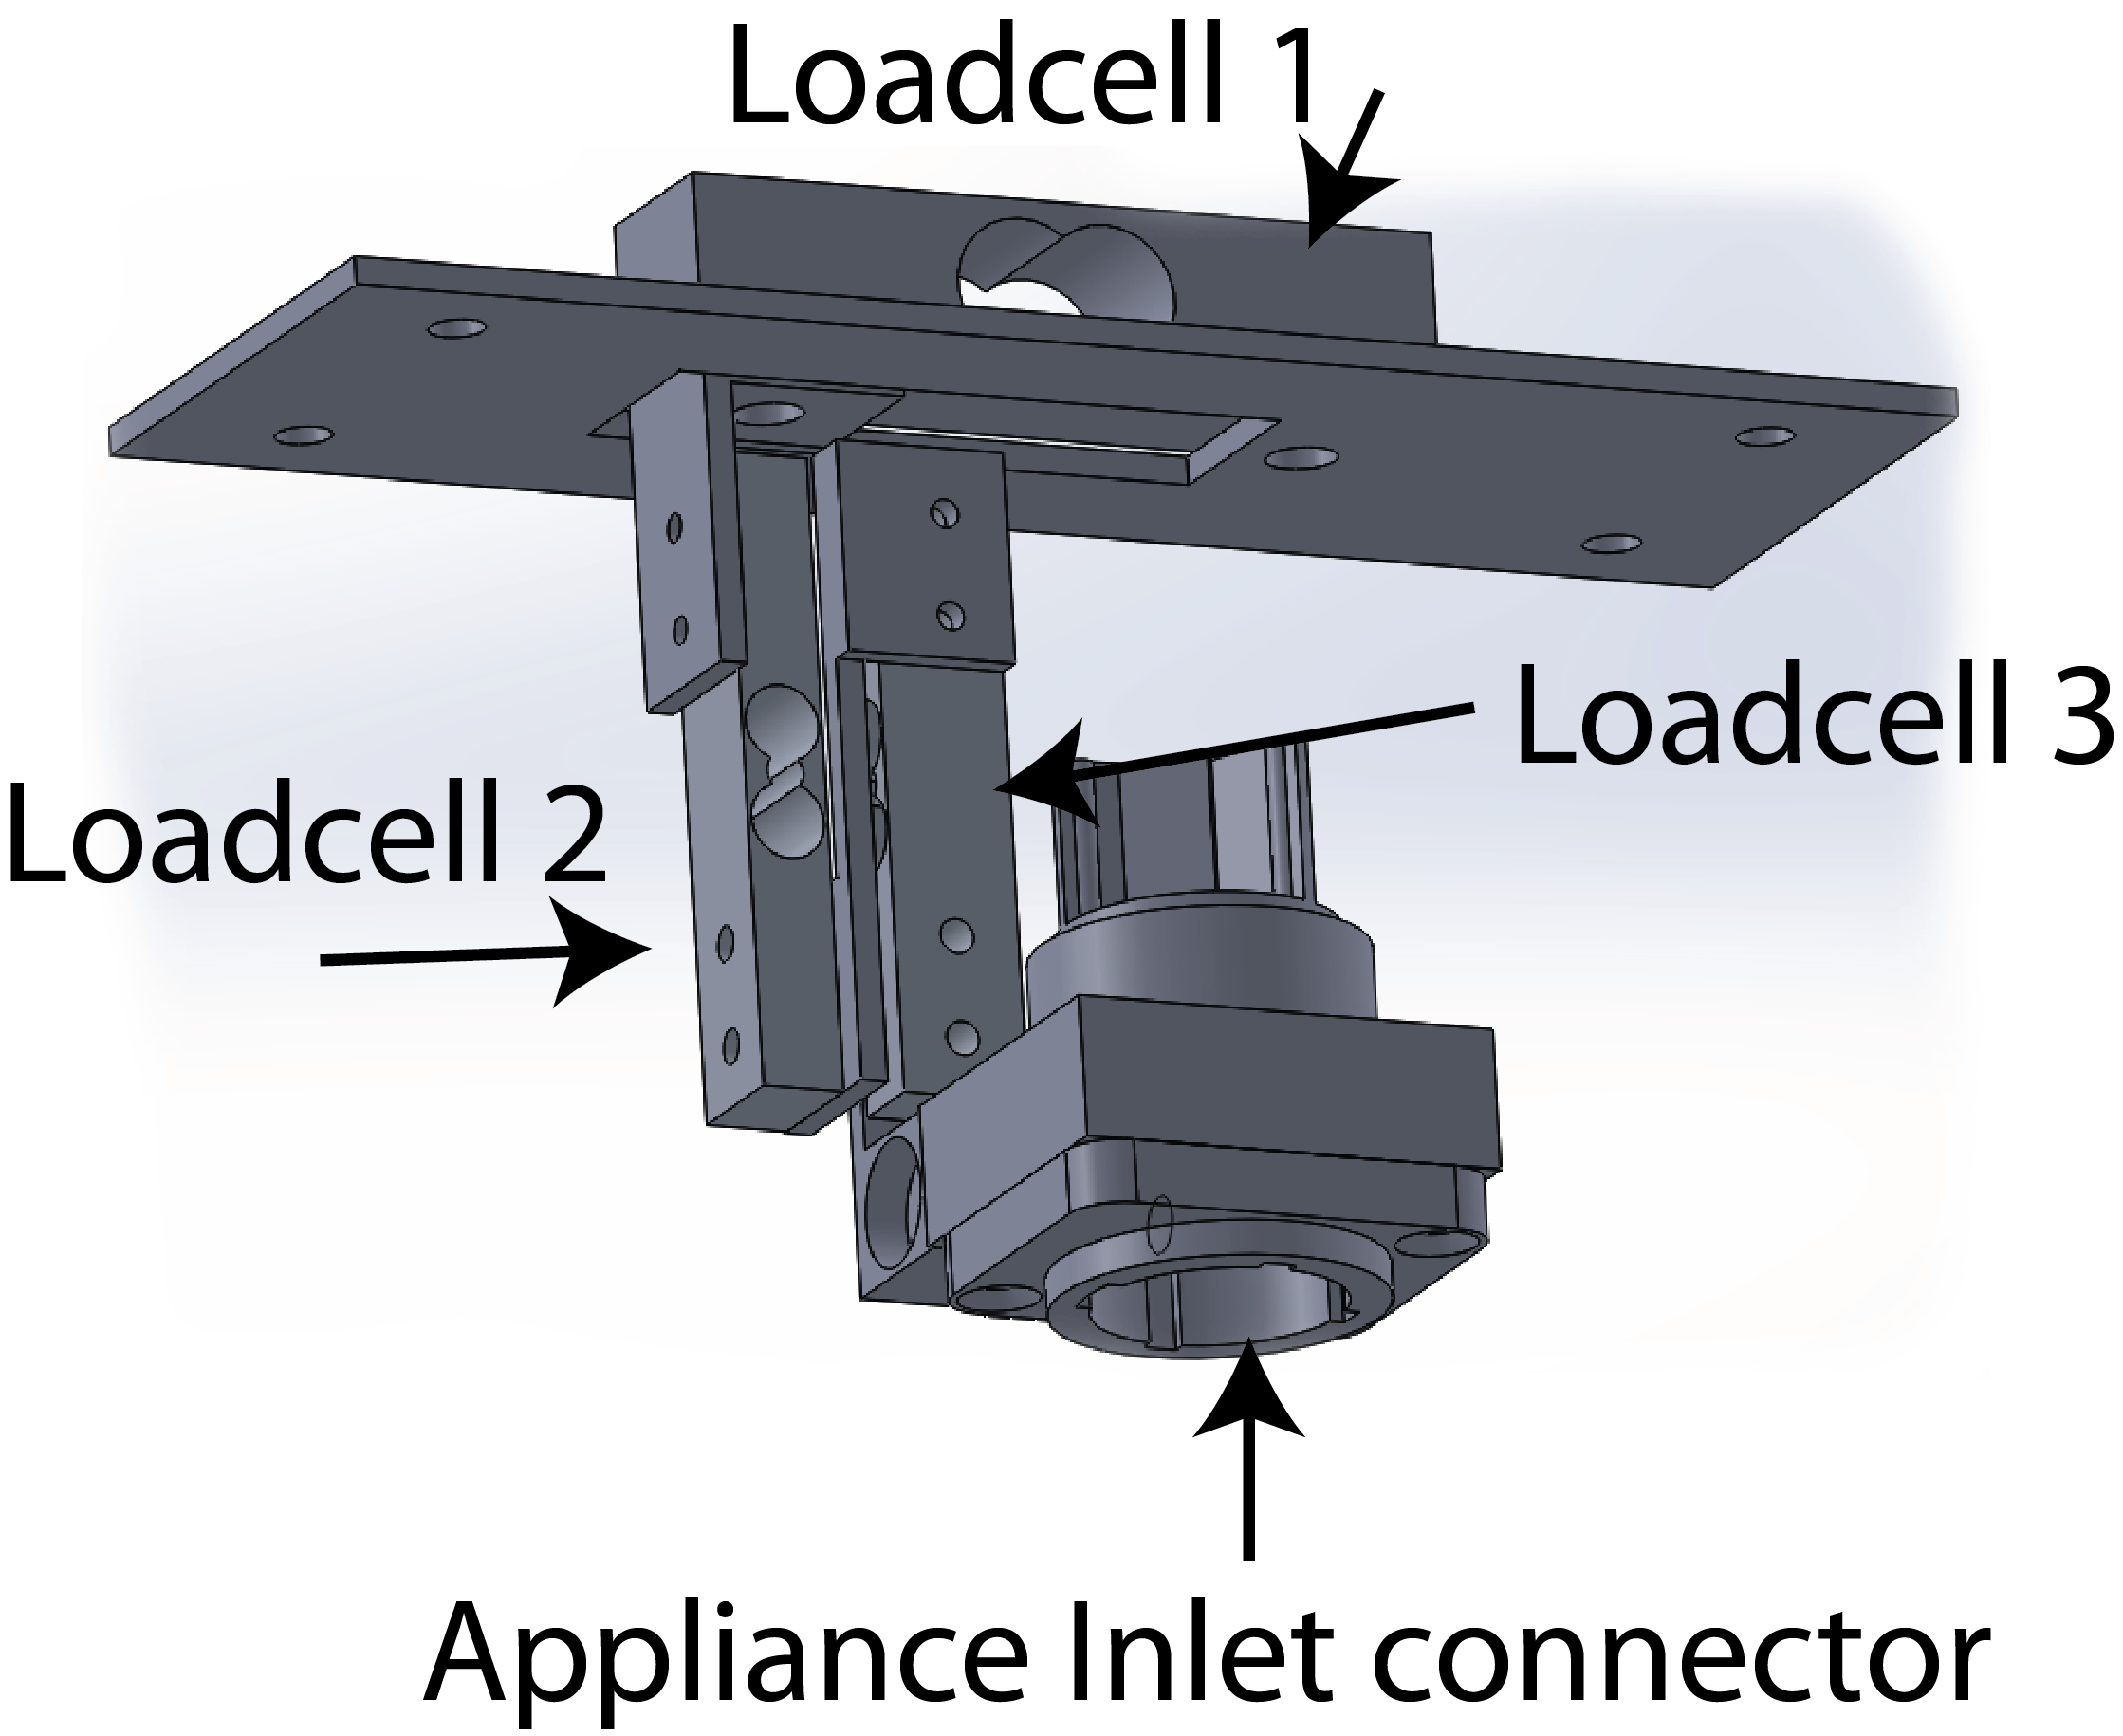
\includegraphics[scale=0.5]{graphics/cad/hexa.png}
\caption{3-axes measuring device for the UAV with appliance inlet connector.}
\end{figure}


\noindent
Second an appliance inlet connector for easy plug-in and unplug is wanted. The connector must be capable to withstand the weight of the cable and the force applied of the UAV. 

\begin{figure}[hbtp]
\centering
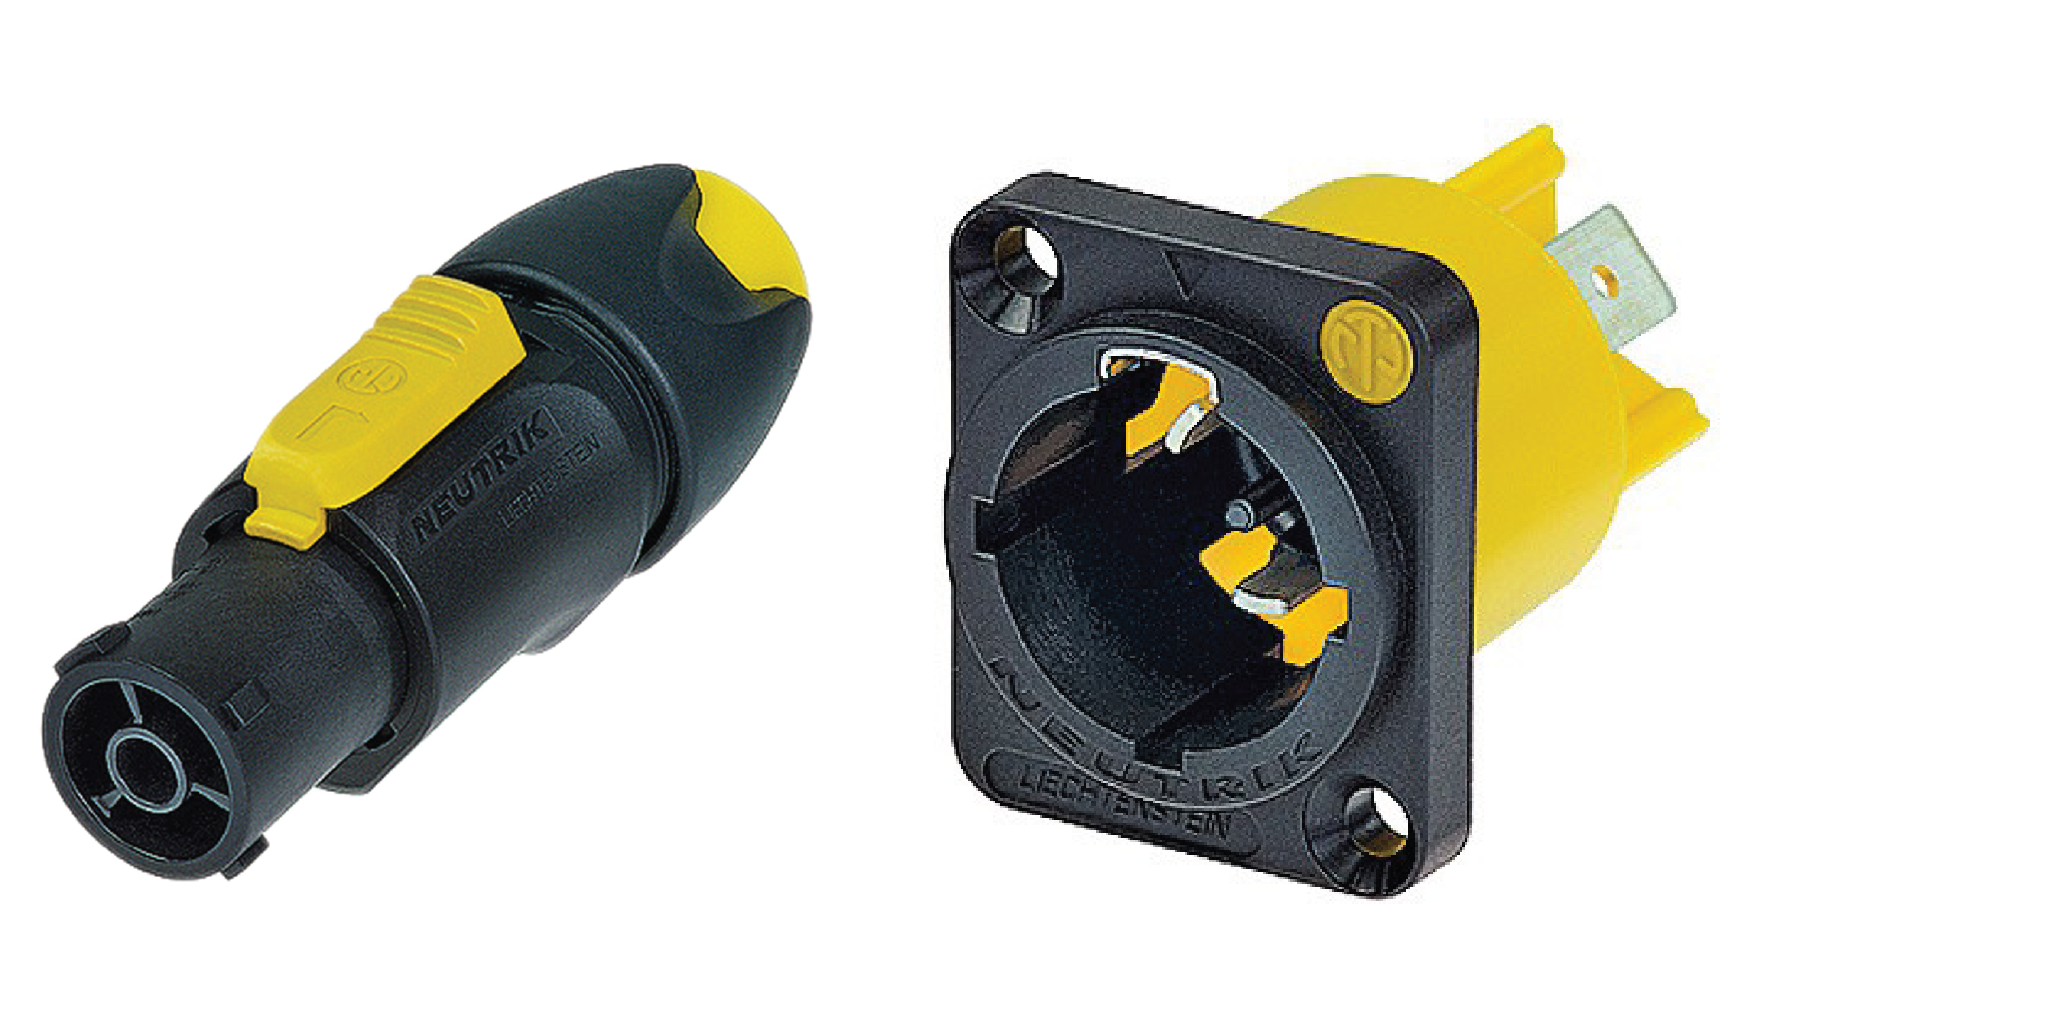
\includegraphics[scale=1]{graphics/Neutrix-True-One.png}
\caption{Neutrix True One appliance connector system.}
\end{figure}



\section{Electrical Design}
From an electrical view there are 2 separate systems, Flight Control System on the UAV and Ground Control Station. The system reading the sensor data on the Ground Control Station has to feed the UAV with the measured data hence the UAV's position controller is running on the UAV. 

\todo{Wire diagram der viser system overview}

\subsection{Ground Station}
The ground station sends data to the UAV system and decides weather to roll cable in or out based on the wanted position. The control of feeding the cable is done by comparing the load on the UAV system to what is expected by the weight of the rolled out amount of cable. If the load is higher then expected more cable are rolled out and vice versa.  
\begin{figure}[hbtp]
\centering
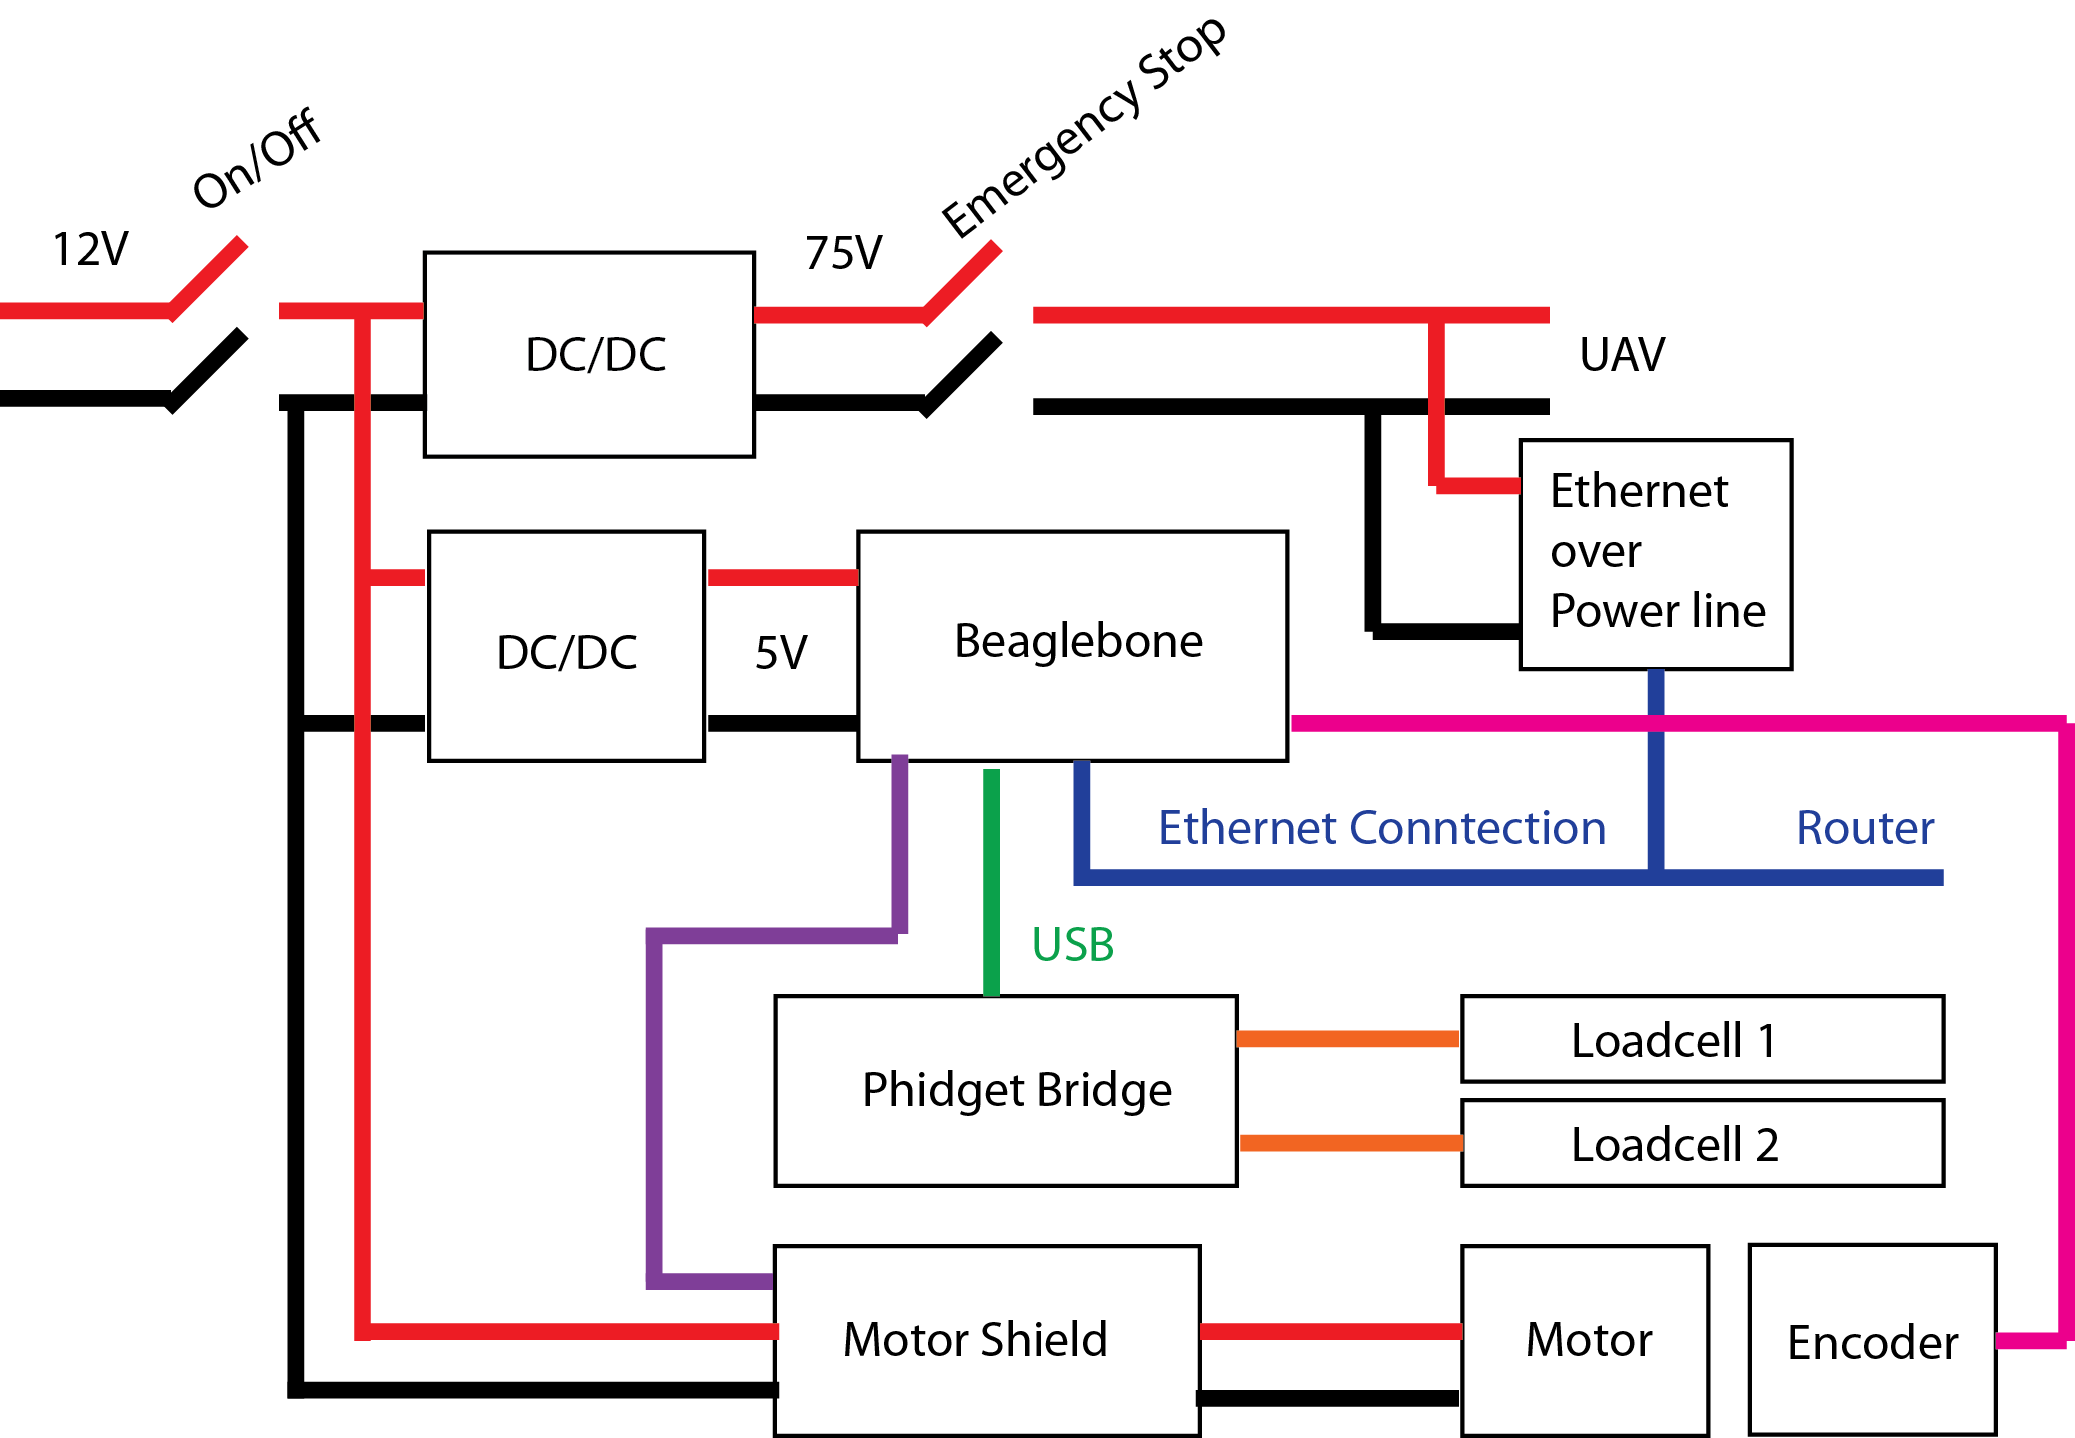
\includegraphics[scale=0.75]{graphics/GCS-eltectrical-overview.png}
\caption{Ground Station electrical overview.}
\end{figure}


\subsection{UAV System}
The system on the UAV measures a 3-axis loadcell connected to a Phigets Bridge. The Phidget Bridge are interfaced via a Beaglebone Black.  

\begin{figure}[hbtp]
\centering
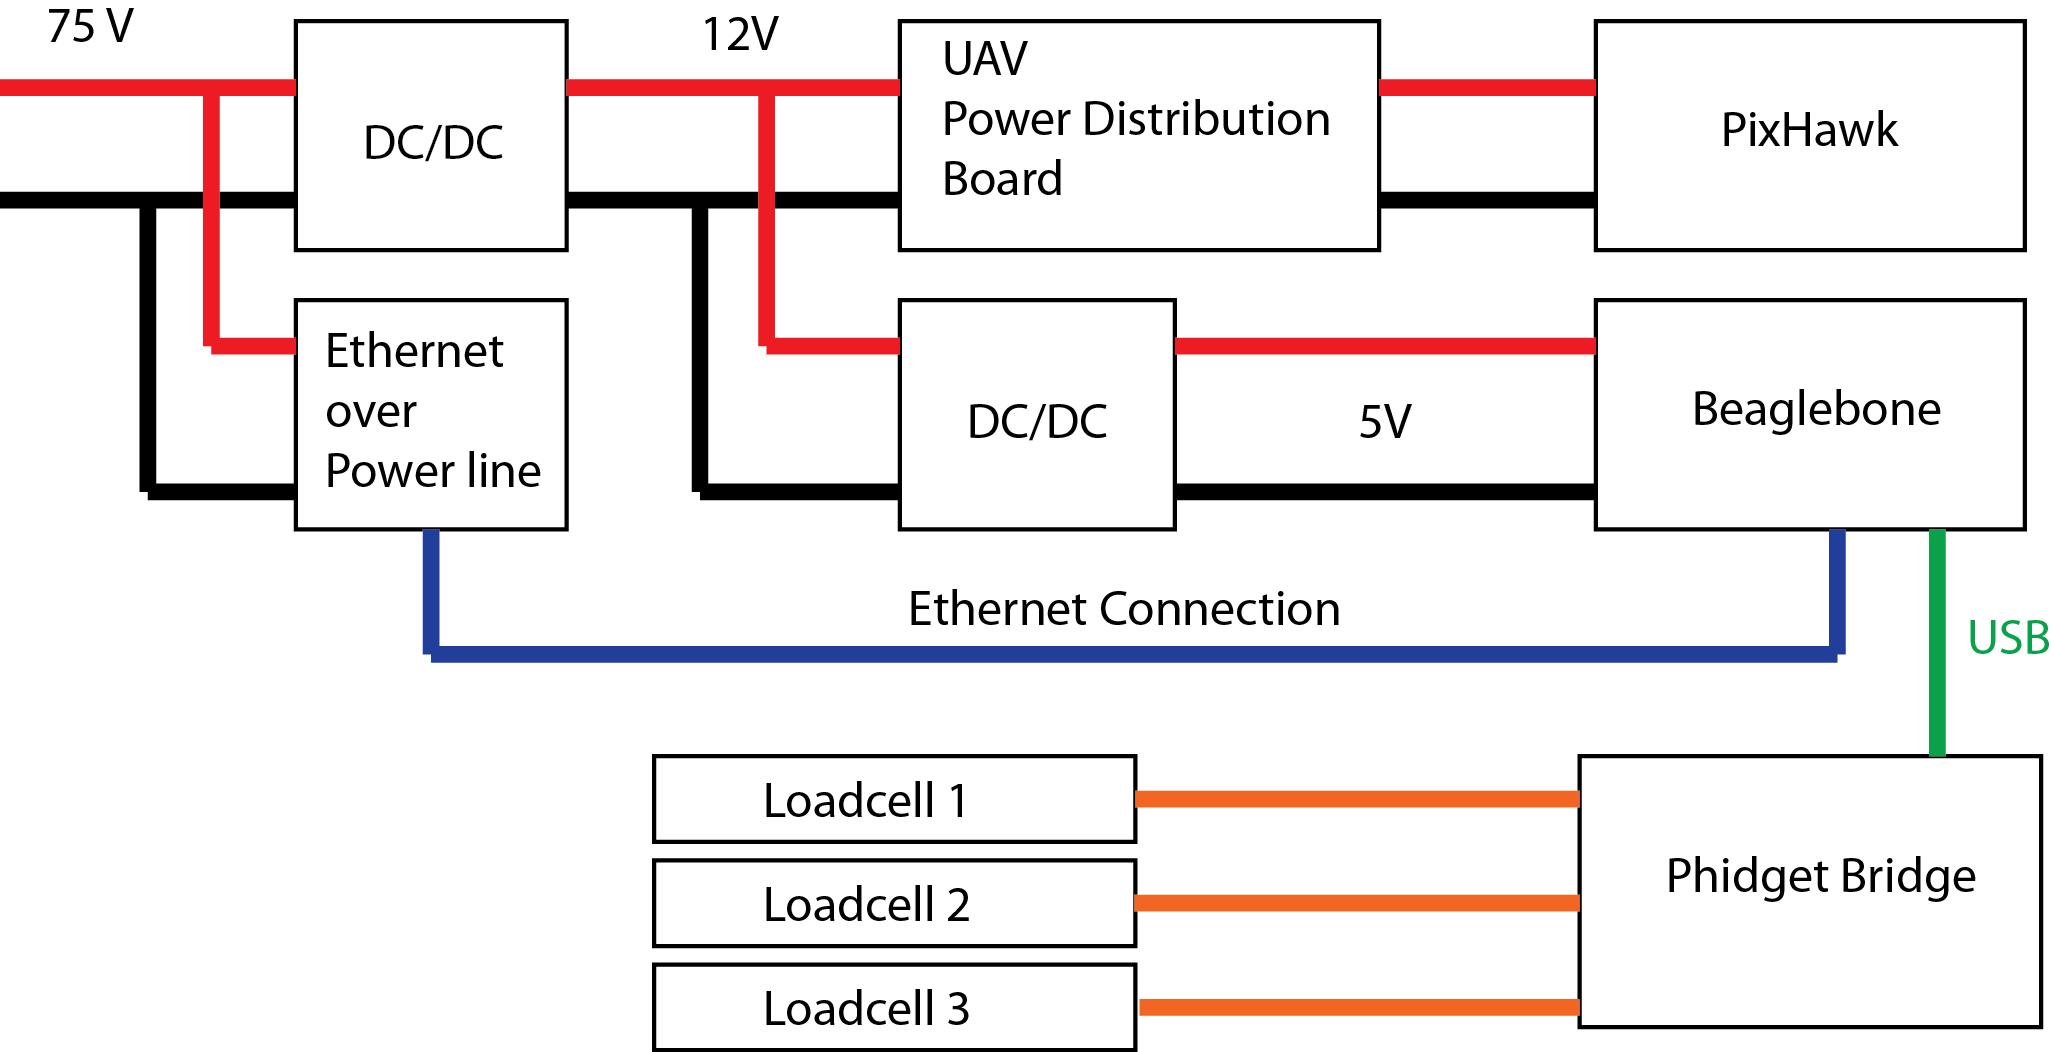
\includegraphics[scale=0.75]{graphics/UAV-electrical-system.png}
\caption{UAV electrical overview.}
\end{figure}



\subsection{Data Connection using Ethernet over Power line}
To connect the UAV to the Ground Station an Ethernet over power line system is used. Ethernet over power line operate by adding a modulated carrier to the wiring system, intended to work on 110-230 volt AC with frequencies in 50-60 Hertz. The AV500 Nano\footnote{Model number: TL-PA411KIT.} system from TP-Link supports speeds up to 500Mbps and works without any configuration needed. Stripping the housing from the electronic and soldering 2 wires on to parallel connect the component to the 75 volt system. 

\begin{figure}[hbtp]
\centering
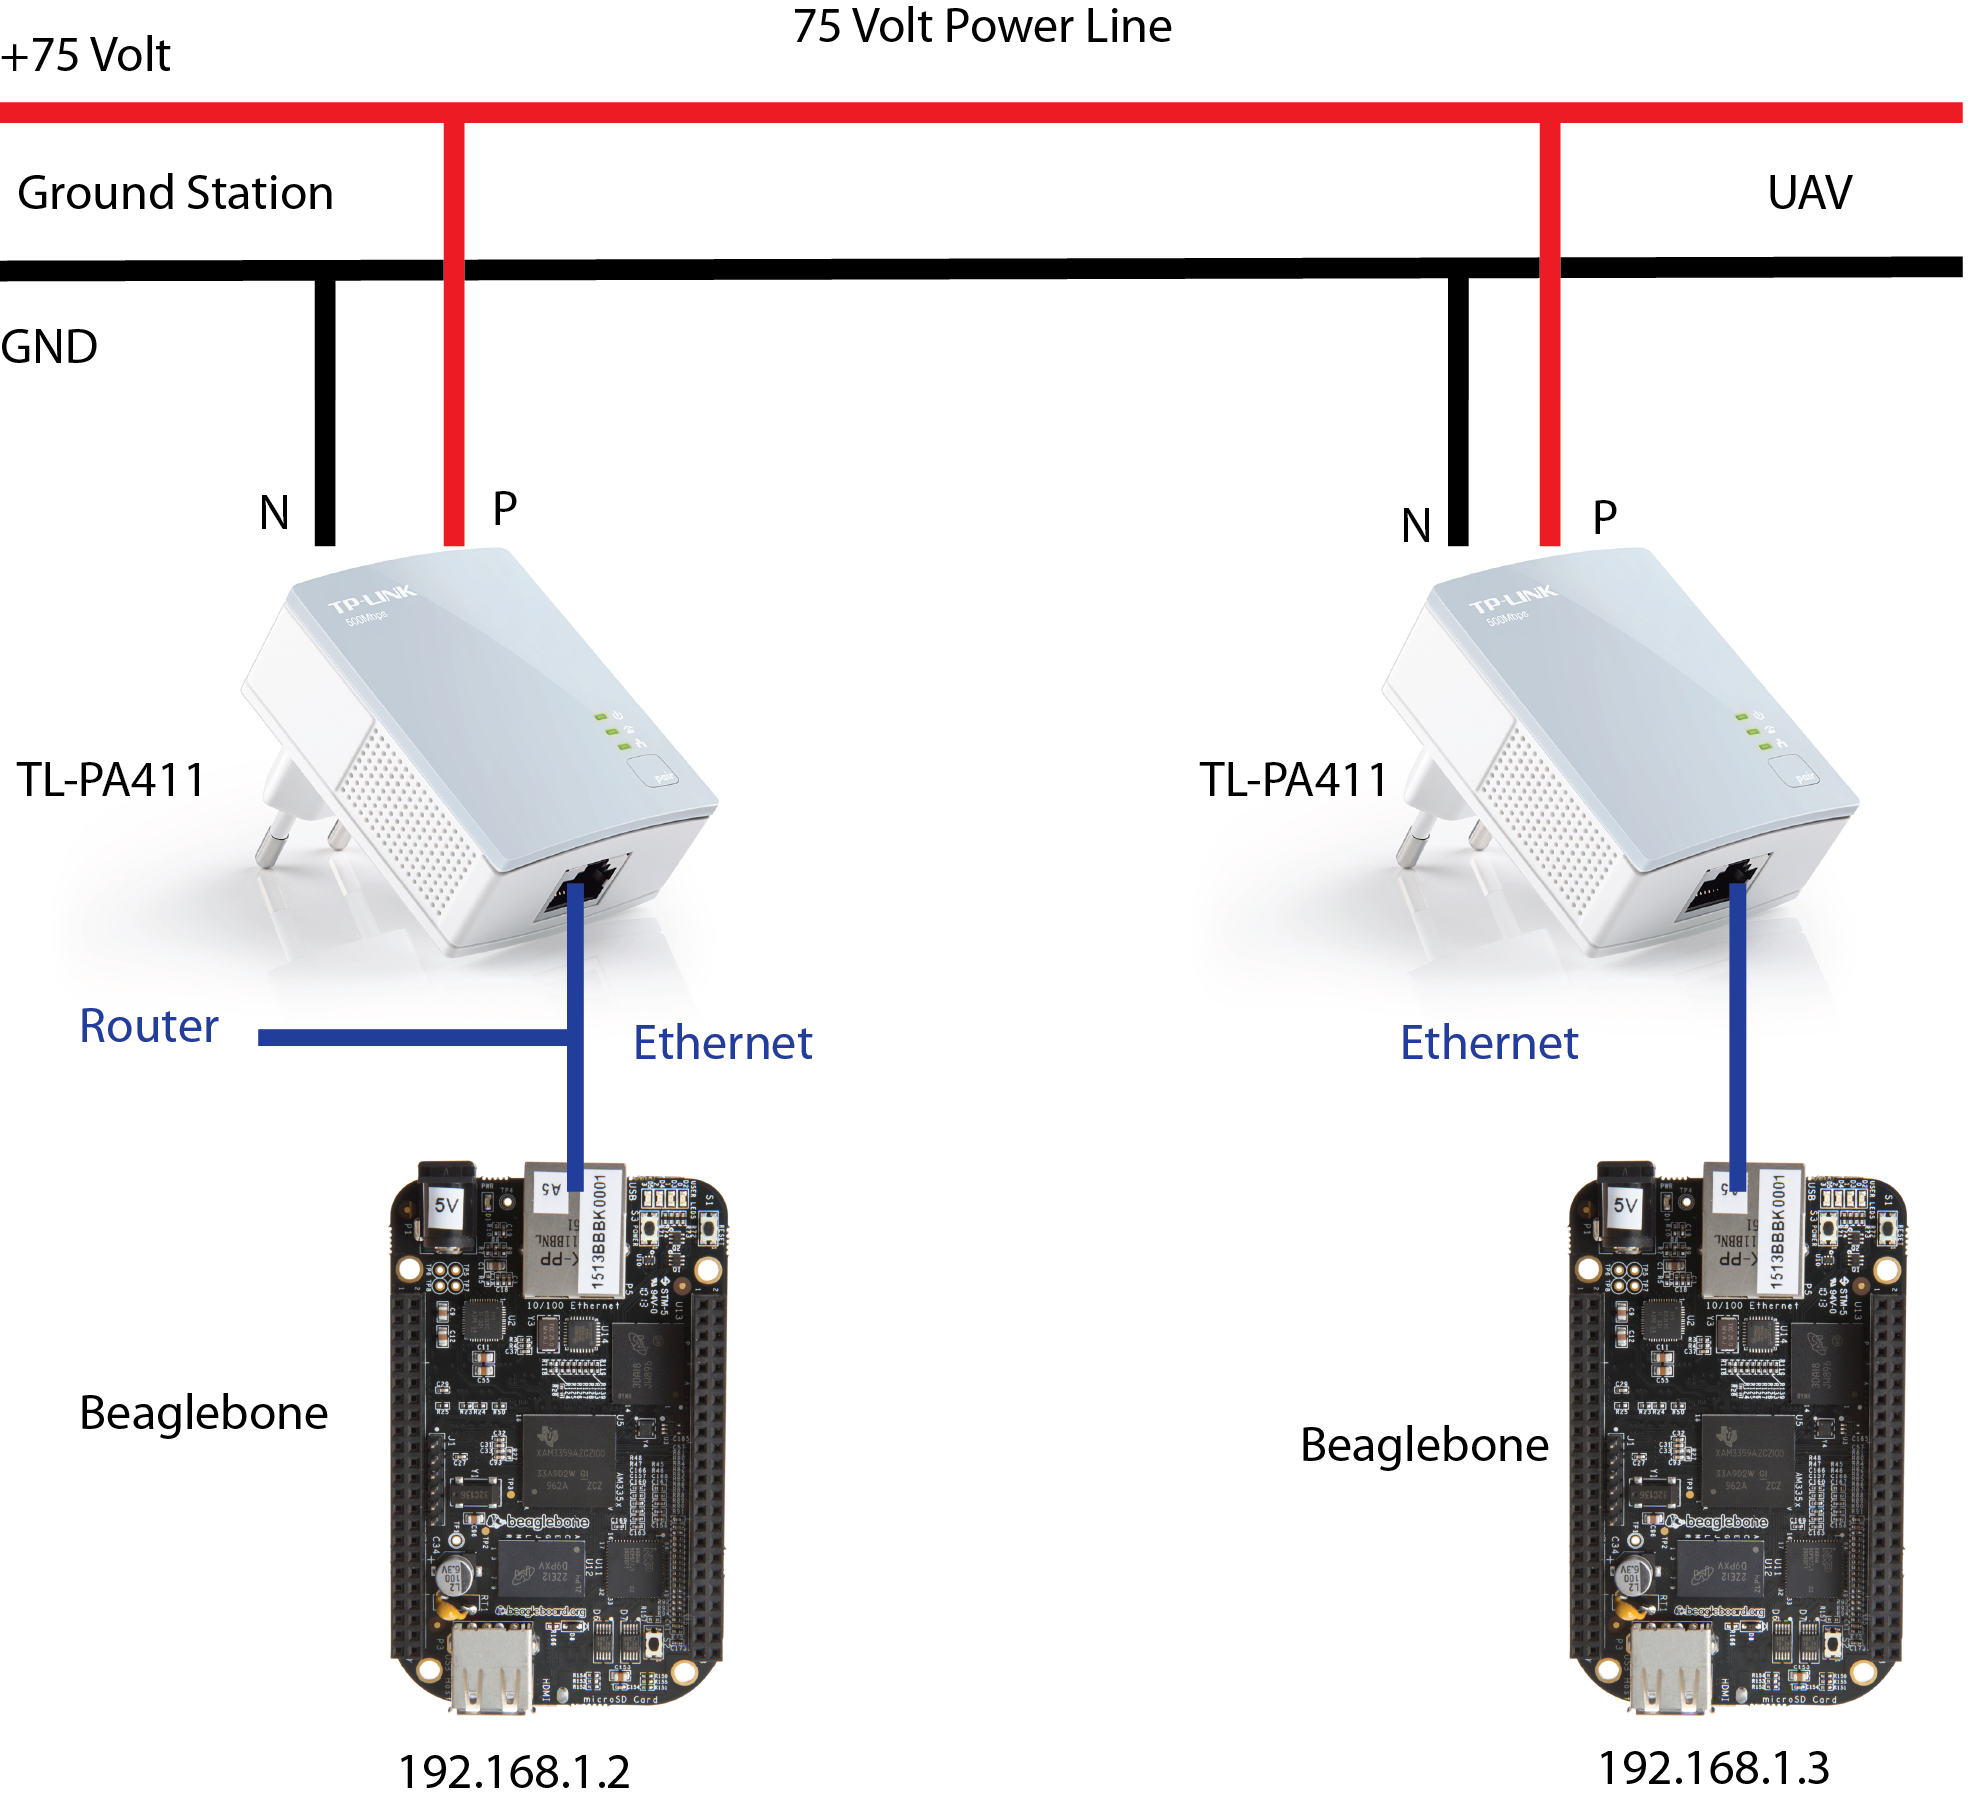
\includegraphics[scale=0.75]{graphics/EthernetLink.png}
\caption{Ethernet over power line setup. Two TL-PA411 is connected to the 75 volt powerline creating an Ethernet over power line connection to the UAV.}
\label{fig:Networking}
\end{figure}



\section{Software design}


\subsection{Flight Control System}


\subsection{Ground Control Station}
